\onecolumn

\begin{center}
	\textbf{\LARGE Supplementary Materials}
\end{center}

\bigskip

\section*{A\quad Architectures and Hyperparameters}

\bigskip

\subsection*{A.1\quad Default Settings}
By default, we chose ReLU, SGD with Adam optimizer, and a learning rate of 0.0001 for networks. Mini-batch size is set to 100 by default but is set to 500 only for CIFAR-100. We evaluated validation performance for \{0.001, 0.01, 0.1, 1, 10, 100\} and chose the one 
with the best performance for each regularizer and condition.
Then, performance was evaluated through five trainings 
using the pre-fixed weight value. In the case of CIFAR-10 and CIFAR-100, 
the last 10,000 instances of 50,000 training data were used as the validation data,
and after the weight values are fixed, the validation data was merged back into training data. All experiments in this work were carried out using TensorFlow 1.5.

\bigskip

\subsection*{A.2\quad MNIST}
For classification tasks, a 6-layer MLP that has 100 hidden units per layer was used. For image reconstruction task, a 6-layer autoencoder was used. The number of hidden units in each layer is 400, 200, 100, 200, 400, and 784 in the order of hidden layers. 

\bigskip

\subsection*{A.3\quad CIFAR-10 and CIFAR-100}
A CNN with four convolutional layers and one fully connected layer was used for both of CIFAR-10 and CIFAR-100. Detailed architecture hyperparameters are shown in Table 6.

\begin{table}[htbp]
\centering
\captionsetup{labelformat=empty}
\caption{Table 6: Default architecture hyperparameters of CIFAR-10/100 CNN model.}
\resizebox{\textwidth}{!}{%
\begin{tabular}{cccccc}
\hline
Layer                 & \# of filters (or units) & Filter size               & Conv. stride & Pooling size              & Pooling stride \\ \hline
Convolutional layer-1 & 32                & 3 $\times$ 3 & 1             & -                         & -              \\
Convolutional layer-2 & 64                & 3 $\times$ 3 & 1             & -                         & -              \\
Max-pooling layer-1   & -                 & -                         & -             & 2 $\times$ 2 & 2              \\
Convolutional layer-3 & 128               & 3 $\times$ 3 & 1             & -                         & -              \\
Max-pooling layer-2   & -                 & -                         & -             & 2 $\times$ 2 & 2              \\
Convolutional layer-4 & 128               & 3 $\times$ 3 & 1             & -                         & -              \\
Max-pooling layer-3   & -                 & -                         & -             & 2 $\times$ 2 & 2 \\ 
Fully connected layer   & 128                 & -                         & -             & - & - \\ \hline             
\end{tabular}
}
\label{table:hyperparameters}
\end{table}



\clearpage

\section*{B\quad Result Details}
\begin{table*}[ht]
\captionsetup{labelformat=empty}
\caption{Table 7: Results for MNIST MLP model. 
The best performing regularizer in each condition (each column) is shown in bold.
For the default condition, the standard values of data size=50k and layer width=100 were used.}
\vskip -0.8in
\begin{center}
\begin{small}
% \begin{sc}
\begin{tabular}{lcccccr}
\hline
\multirow{2}{*}{Regularizer} & \multirow{2}{*}{Default} & \multicolumn{2}{c}{Data size}      & \multicolumn{2}{c}{Layer width}     \\ \cmidrule{3-6} 
                             &                          & 1k               & 5k              & 2                & 8                \\ \hline
Baseline                     & $2.85 \pm 0.11$          & $11.41 \pm 0.19$ & $6.00 \pm 0.07$ & $31.62 \pm 0.07$ & $10.52 \pm 0.57$ \\ \hline
L1W                          & $2.85 \pm 0.06$          & $11.64 \pm 0.27$ & $5.96 \pm 0.11$ & $31.67 \pm 0.15$ & $11.02 \pm 0.58$ \\ 
L2W                          & $3.02 \pm 0.40$          & $11.38 \pm 0.18$ & $5.86 \pm 0.10$ & $31.66 \pm 0.13$ & $10.65 \pm 0.23$ \\ \hline
% Dropout                      & $2.70 \pm 0.08$          & \bgcblack{$10.29 \pm 0.23$} & \bgcblack{$5.59 \pm 0.11$} & $62.09 \pm 1.32$ & $13.94 \pm 1.05$ \\ \hline
% BN                           & $2.81 \pm 0.12$          & $10.81 \pm 0.04$ & \bgcbb{$5.60 \pm 0.10$} & $42.08 \pm 0.93$ & \bgcblack{$7.51 \pm 0.58$}  \\ \hline
% L1R                          & \bgcblack{$2.35 \pm 0.08$}          & $11.60 \pm 0.20$ & $6.20 \pm 0.13$ & $64.39 \pm 0.26$ & $88.65 \pm 0.00$ \\ \hline
CR (DeCov)                           & $2.50 \pm 0.05$          & $11.63 \pm 0.24$ & $6.05 \pm 0.06$ & $34.80 \pm 0.25$ & $10.25 \pm 0.74$ \\ 
cw-CR                        & $2.49 \pm 0.10$          & $10.62 \pm 0.05$ & \pmb{$5.80 \pm 0.15$} & $31.50 \pm 0.11$ & $10.81 \pm 1.11$ \\ 
VR                           & $2.65 \pm 0.11$          & $14.42 \pm 0.14$ & $6.90 \pm 0.22$ & $32.39 \pm 0.13$ & \pmb{$9.22 \pm 0.28$}  \\ 
cw-VR                        & \pmb{$2.42 \pm 0.06$}    & \pmb{$10.44 \pm 0.18$} & $5.90 \pm 0.12$ & \pmb{$30.34 \pm 0.06$} & $10.01 \pm 0.63$ \\ 
\hline
\end{tabular}
\label{appendix_mnist}
% \end{sc}
\end{small}
\end{center}
\vskip 0.1in
% \end{table*}
\bigskip

% \begin{table*}[htbp]
\centering
\captionsetup{labelformat=empty}
\caption{Table 8: Results for CIFAR-10 CNN model. 
The best performing regularizer in each condition (each column) is shown in bold.
% The best performing regularizers in each condition (each column) are highlighted in green, 
% and the best performing one is shown in bold.
For the default condition, the standard values of data size=50k and layer width=128 were used 
and Adam optimizer was applied.}
% \begin{sc}
\vskip -0.8in
\begin{center}
% \begin{small}
\resizebox{\textwidth}{!}{%
\begin{tabular}{cccccccc}
\hline
\multirow{2}{*}{Regularizer} & \multirow{2}{*}{Default} & \multicolumn{2}{c}{Data size}       & \multicolumn{2}{c}{Layer width} & \multicolumn{2}{c}{Optimizer}    \\ \cmidrule{3-8}
                             &                          & 1k               & 5k               & 32                & 512         & {Momentum} & {RMSProp}       \\ \midrule
Baseline                     & $26.64 \pm 0.16$         & $56.07 \pm 0.36$ & $43.95 \pm 0.43$ & $28.54 \pm 0.63$ & $28.52 \pm 1.06$             & $25.78 \pm 0.37$ & $28.52 \pm 1.21$ \\ \hline
L1W                          & $26.46 \pm 0.39$         & $56.64 \pm 0.91$ & $44.32 \pm 0.66$ & $28.65 \pm 1.14$ & $27.96 \pm 0.72$             & $25.73 \pm 0.40$ & $28.30 \pm 0.99$ \\
L2W                          & $25.71 \pm 0.98$            & $56.57 \pm 0.22$ & $44.87 \pm 0.81$ & $28.54 \pm 0.30$  & $27.79 \pm 0.83$    & $26.35 \pm 0.54$ & $28.02 \pm 0.88$ \\ \hline
% Dropout                      & $29.25 \pm 0.75$         & $56.11 \pm 0.83$ & $44.78 \pm 0.41$ & $27.66 \pm 0.51$ & $28.43 \pm 0.88$             & $25.95 \pm 0.57$ & $27.69 \pm 0.38$ \\
% BN                           & $27.69 \pm 0.69$         & $56.49 \pm 0.32$ & $43.75 \pm 0.76$ & $28.83 \pm 0.47$ & $28.20 \pm 0.40$             & $25.50 \pm 0.55$ & $28.38 \pm 0.86$ \\
% L1R                          & \bgcblack{$24.66 \pm 0.61$}         & \bgcbb{$52.39 \pm 0.99$} & \bgcblack{$40.92 \pm 0.33$} & \bgcbb{$25.49 \pm 0.61$} & $27.81 \pm 0.43$     & \bgcbb{$25.13 \pm 0.52$}  & \bgcbb{$26.49 \pm 0.96$}\\
CR (DeCov)                          & $24.96 \pm 0.63$         & $57.40 \pm 2.11$  & $45.16 \pm 0.94$ & $26.45 \pm 0.22$ & $28.65 \pm 1.21$            & $26.72 \pm 0.61$   & $27.94 \pm 0.43$  \\
cw-CR                        & $22.99 \pm 0.58$         & $53.50 \pm 1.05$  & \pmb{$42.15 \pm 0.64$} & $26.40 \pm 0.62$  & $28.54 \pm 1.01$    & $25.93 \pm 0.59$    & $27.77 \pm 0.88$  \\
VR                           & \pmb{$21.44 \pm 0.88$}         & $53.90 \pm 0.97$  & $42.33 \pm 0.57$ & \pmb{$24.96 \pm 0.26$} & $26.61 \pm 0.47$ & $25.01 \pm 0.41$    & \pmb{$26.06 \pm 0.72$}  \\
cw-VR                        & $21.58 \pm 0.21$         & \pmb{$51.93 \pm 1.09$} & $43.00 \pm 0.95$    & $25.81 \pm 0.64$ & \pmb{$26.46 \pm 0.25$}     &  \pmb{$24.42 \pm 0.31$}   & $26.19 \pm 1.35$  \\
\hline
\end{tabular}%
}
\label{cifar10_dependency}
% \end{small}
\end{center}
% \end{sc}
\vskip 0.1in

% \end{table*}
\bigskip

% \begin{table*}[htbp]

\centering
    \captionsetup{labelformat=empty}
\caption{Table 9: Results for CIFAR-100 CNN model. The best performing regularizer in each condition (each column) is shown in bold. For the default condition, the standard values of data size=50k, layer width=128, and number of classes=100 were used.}
% \begin{sc}
\vskip -0.8in
\begin{center}
% \begin{small}
\resizebox{\textwidth}{!}{%
\begin{tabular}{ccccccccc}
\hline
\multirow{2}{*}{Regularizer} & \multirow{2}{*}{Default} & \multicolumn{2}{c}{Data Size}       & \multicolumn{2}{c}{Layer Width}     & \multicolumn{3}{c}{Classes}                            \\ \cmidrule{3-9}
                             &                          & 1k               & 5k               & 32               & 512              & 4                & 16               & 64               \\ \midrule
Baseline                     & $61.26 \pm 0.52$         & $90.89 \pm 0.30$ & $82.21 \pm 0.72$ & $62.41 \pm 0.34$ & $61.30 \pm 0.64$  & \pmb{$24.95 \pm 2.36$} & $45.75 \pm 0.73$ & $58.02 \pm 0.40$  \\ \hline
L1W                          & $60.97 \pm 0.64$         & $91.33 \pm 0.37$ & $82.3 \pm 0.6$   & $62.23 \pm 0.58$ & $60.92 \pm 0.47$ & $26.75 \pm 2.04$ & $45.08 \pm 1.53$ & $58.08 \pm 1.18$ \\
L2W                          & $60.23 \pm 0.31$         & $90.53 \pm 0.39$ & $82.05 \pm 0.70$  & $62.78 \pm 0.36$ & $61.55 \pm 0.99$ & $26.90 \pm 1.24$  & $45.28 \pm 1.59$ & $57.47 \pm 0.66$ \\ \hline
% Dropout                      & $63.88 \pm 0.72$         & \bgcblack{$90.22 \pm 0.48$} & \bgcbb{$81.68 \pm 0.81$} & $64.08 \pm 0.99$ & $64.31 \pm 0.37$ & $25.60 \pm 1.08$  & $45.73 \pm 1.57$ & $59.14 \pm 0.46$ \\
% BN                           & $60.93 \pm 0.39$         & $91.18 \pm 0.36$ & \bgcbb{$82.01 \pm 0.58$} & \bgcbb{$62.18 \pm 1.49$} & $62.16 \pm 0.57$ & $26.10 \pm 1.65$  & $44.55 \pm 1.43$ & $57.72 \pm 0.66$ \\
% L1R                          & \bgcblack{$56.03 \pm 0.81$}         & $91.15 \pm 0.35$ & \bgcbb{$81.98 \pm 0.47$} & \bgcbb{$61.11 \pm 0.31$} & \bgcblack{$56.46 \pm 0.62$} & \bgcblack{$22.20 \pm 1.27$}  & \bgcbb{$42.51 \pm 1.43$} & \bgcblack{$53.65 \pm 1.00$}    \\
CR (DeCov)                          & $59.88 \pm 0.50$         & $91.70 \pm 0.14$  & $82.47 \pm 0.41$ & \pmb{$60.47 \pm 0.63$} & $60.70 \pm 0.94$  & $27.25 \pm 1.51$ & $44.55 \pm 1.10$  & $56.76 \pm 0.86$ \\
cw-CR                        & $57.03 \pm 0.73$         & $90.85 \pm 0.29$ & $81.29 \pm 0.62$ & $61.41 \pm 0.67$ & $58.02 \pm 0.25$ & $26.35 \pm 1.04$ & $43.50 \pm 1.21$  & $54.24 \pm 0.64$ \\ 
VR                           & $57.68 \pm 0.94$         & $91.43 \pm 0.32$ & $81.85 \pm 0.38$ & $61.35 \pm 0.45$ & \pmb{$56.87 \pm 0.74$} & $26.10 \pm 1.81$  & $42.33 \pm 1.03$ & $54.32 \pm 0.40$  \\
cw-VR                        & \pmb{$56.75 \pm 0.64$}   & \pmb{$90.45 \pm 0.22$} & \pmb{$81.03 \pm 0.57$} & $60.67 \pm 0.59$ & $56.91 \pm 0.73$ & $26.40 \pm 1.08$  & \pmb{$41.38 \pm 0.53$} & \pmb{$54.23 \pm 1.06$} \\ \hline

\end{tabular}%
}
\label{cifar100_dependency}
% \end{small}
\end{center}
% \end{sc}
\vskip 0.1in
% \end{table*}

% \end{table*}
\bigskip

% \begin{table*}[htbp]

% \begin{table}[t]
\centering
\captionsetup{labelformat=empty}
\caption{Table 10: Mean squared error of deep autoencoder.}
% \vskip -0.2in
\begin{tabular}{cc}
\hline
Regularizer & Mean Squared Error                       \\ \hline
Baseline    & $1.44 \times 10^{-2} \pm 3.36 \times 10^{-4} $                        \\ \hline
CR          & $1.29 \times 10^{-2} \pm 2.44 \times 10^{-4} $                        \\ 
cw-CR       & $1.22 \times 10^{-2} \pm 3.63 \times 10^{-4} $                        \\ 
VR          & $1.29 \times 10^{-2} \pm 5.16 \times 10^{-4} $                        \\
cw-VR       & \pmb{$1.19 \times 10^{-2} \pm 2.48 \times 10^{-4} $}                  \\ \hline
\end{tabular}
\label{table:autoencoder}
\vskip -1.2in
\end{table*}

\clearpage


\section*{C\quad Principal Component Analysis of Learned Representations}
% L1W and L2W are excluded because their figures are not distinct to the baseline. See page 2.

\begin{figure}[htbp]
% \vskip -0.6in
    \centering
    \quad\subfloat[Baseline (Before ReLU)]{{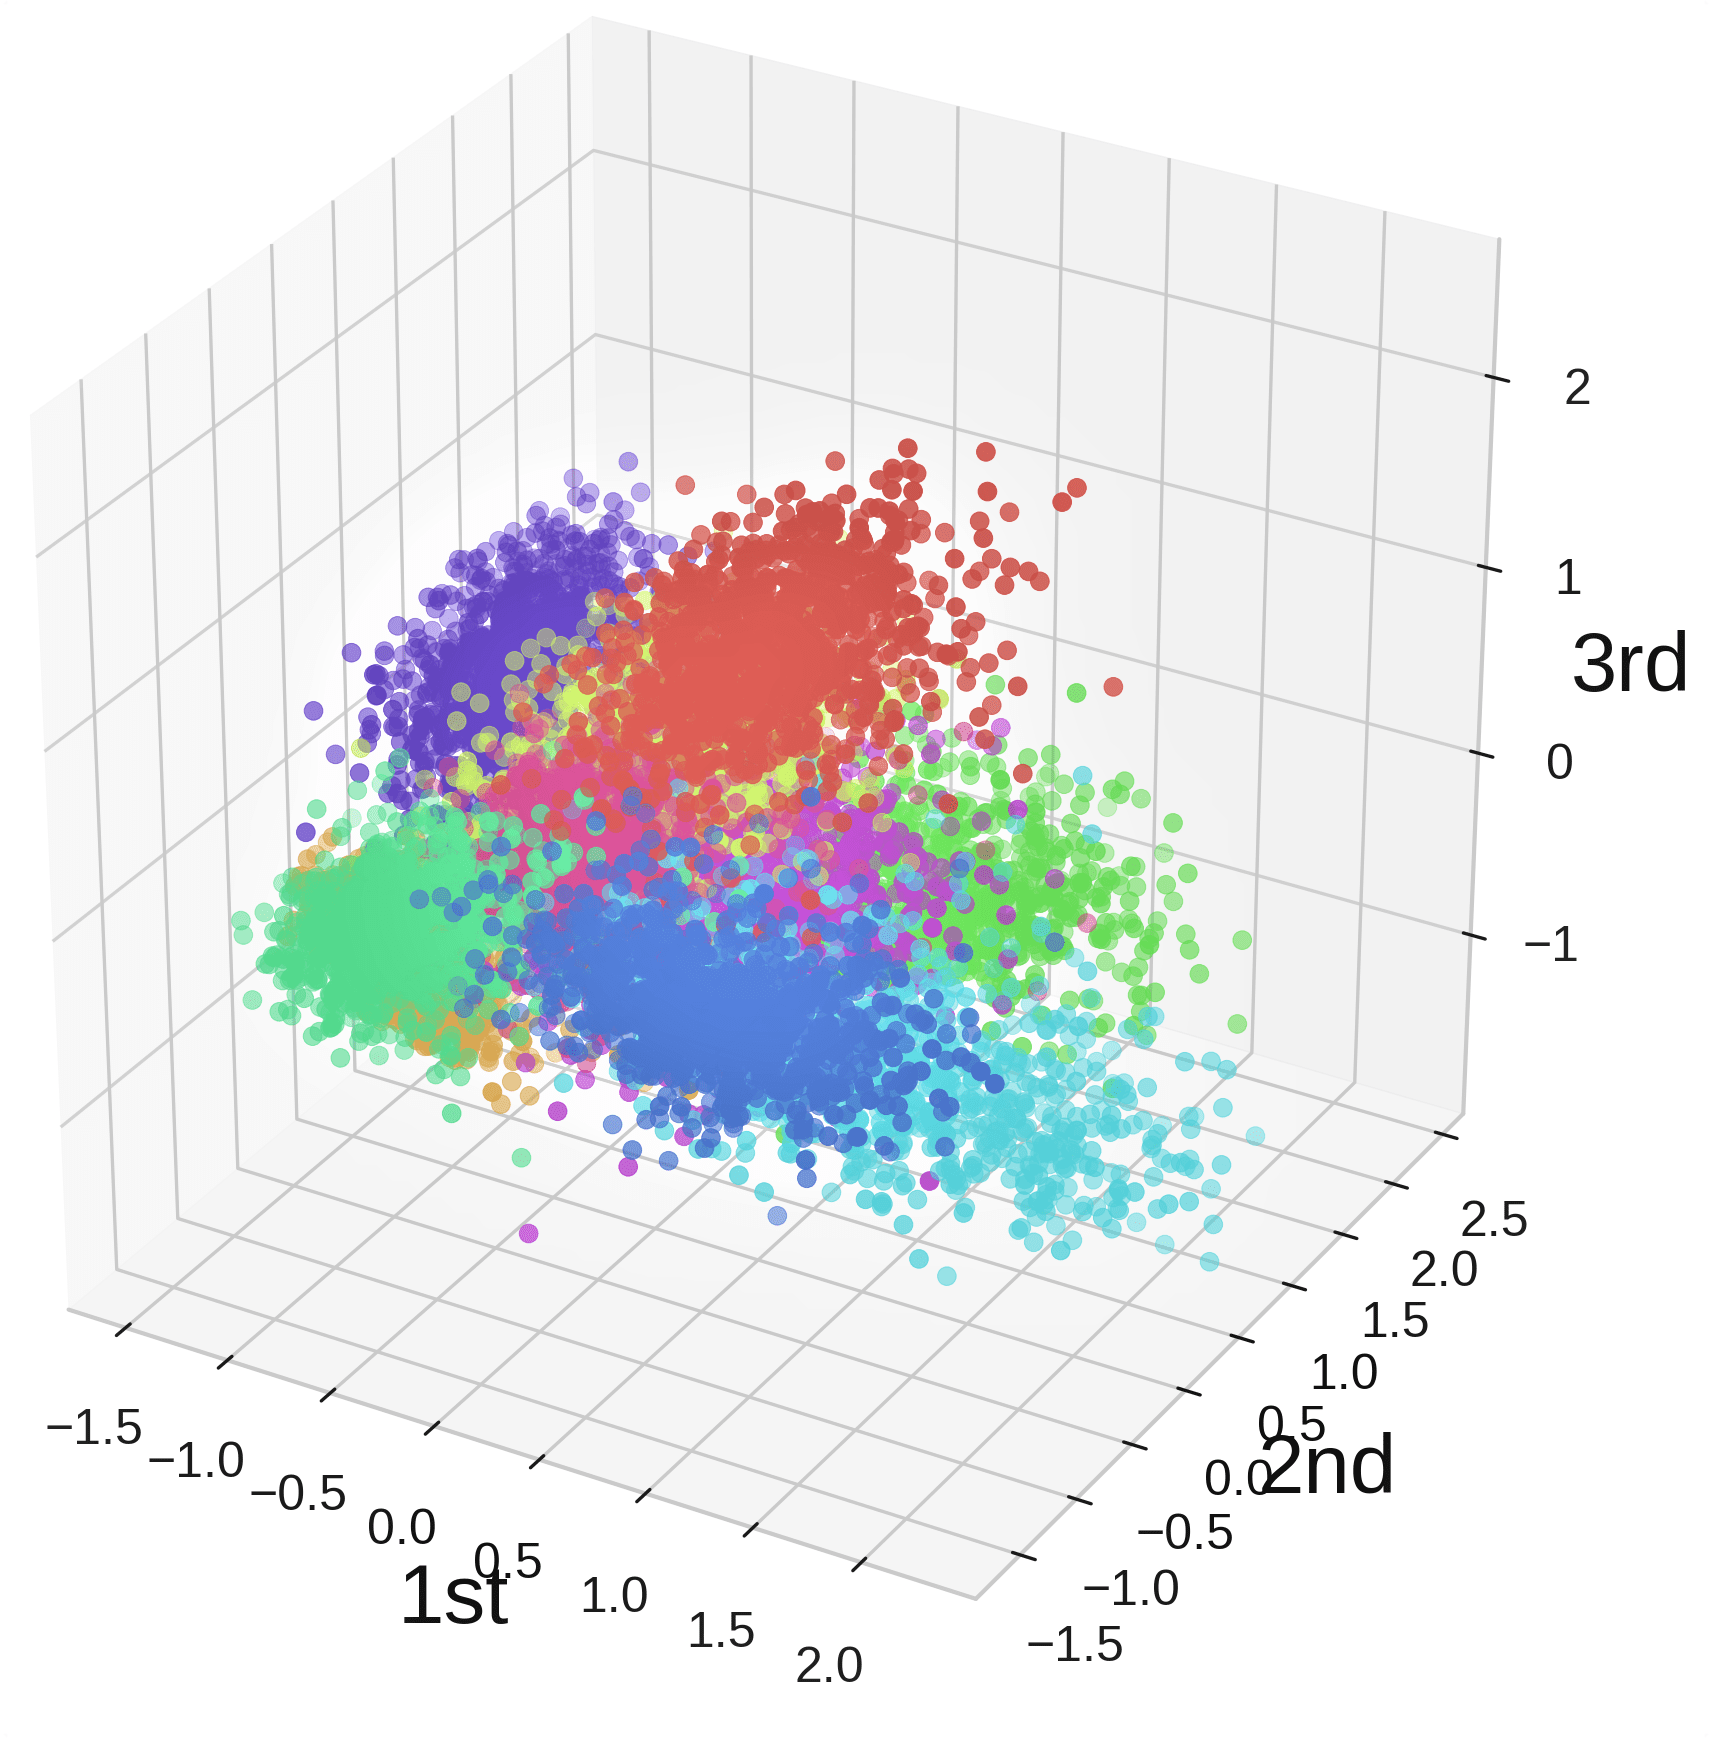
\includegraphics[width=4.1cm]{none_fc5.png} }}%
    \qquad\qquad\qquad\quad
    \subfloat[Baseline (After ReLU)]{{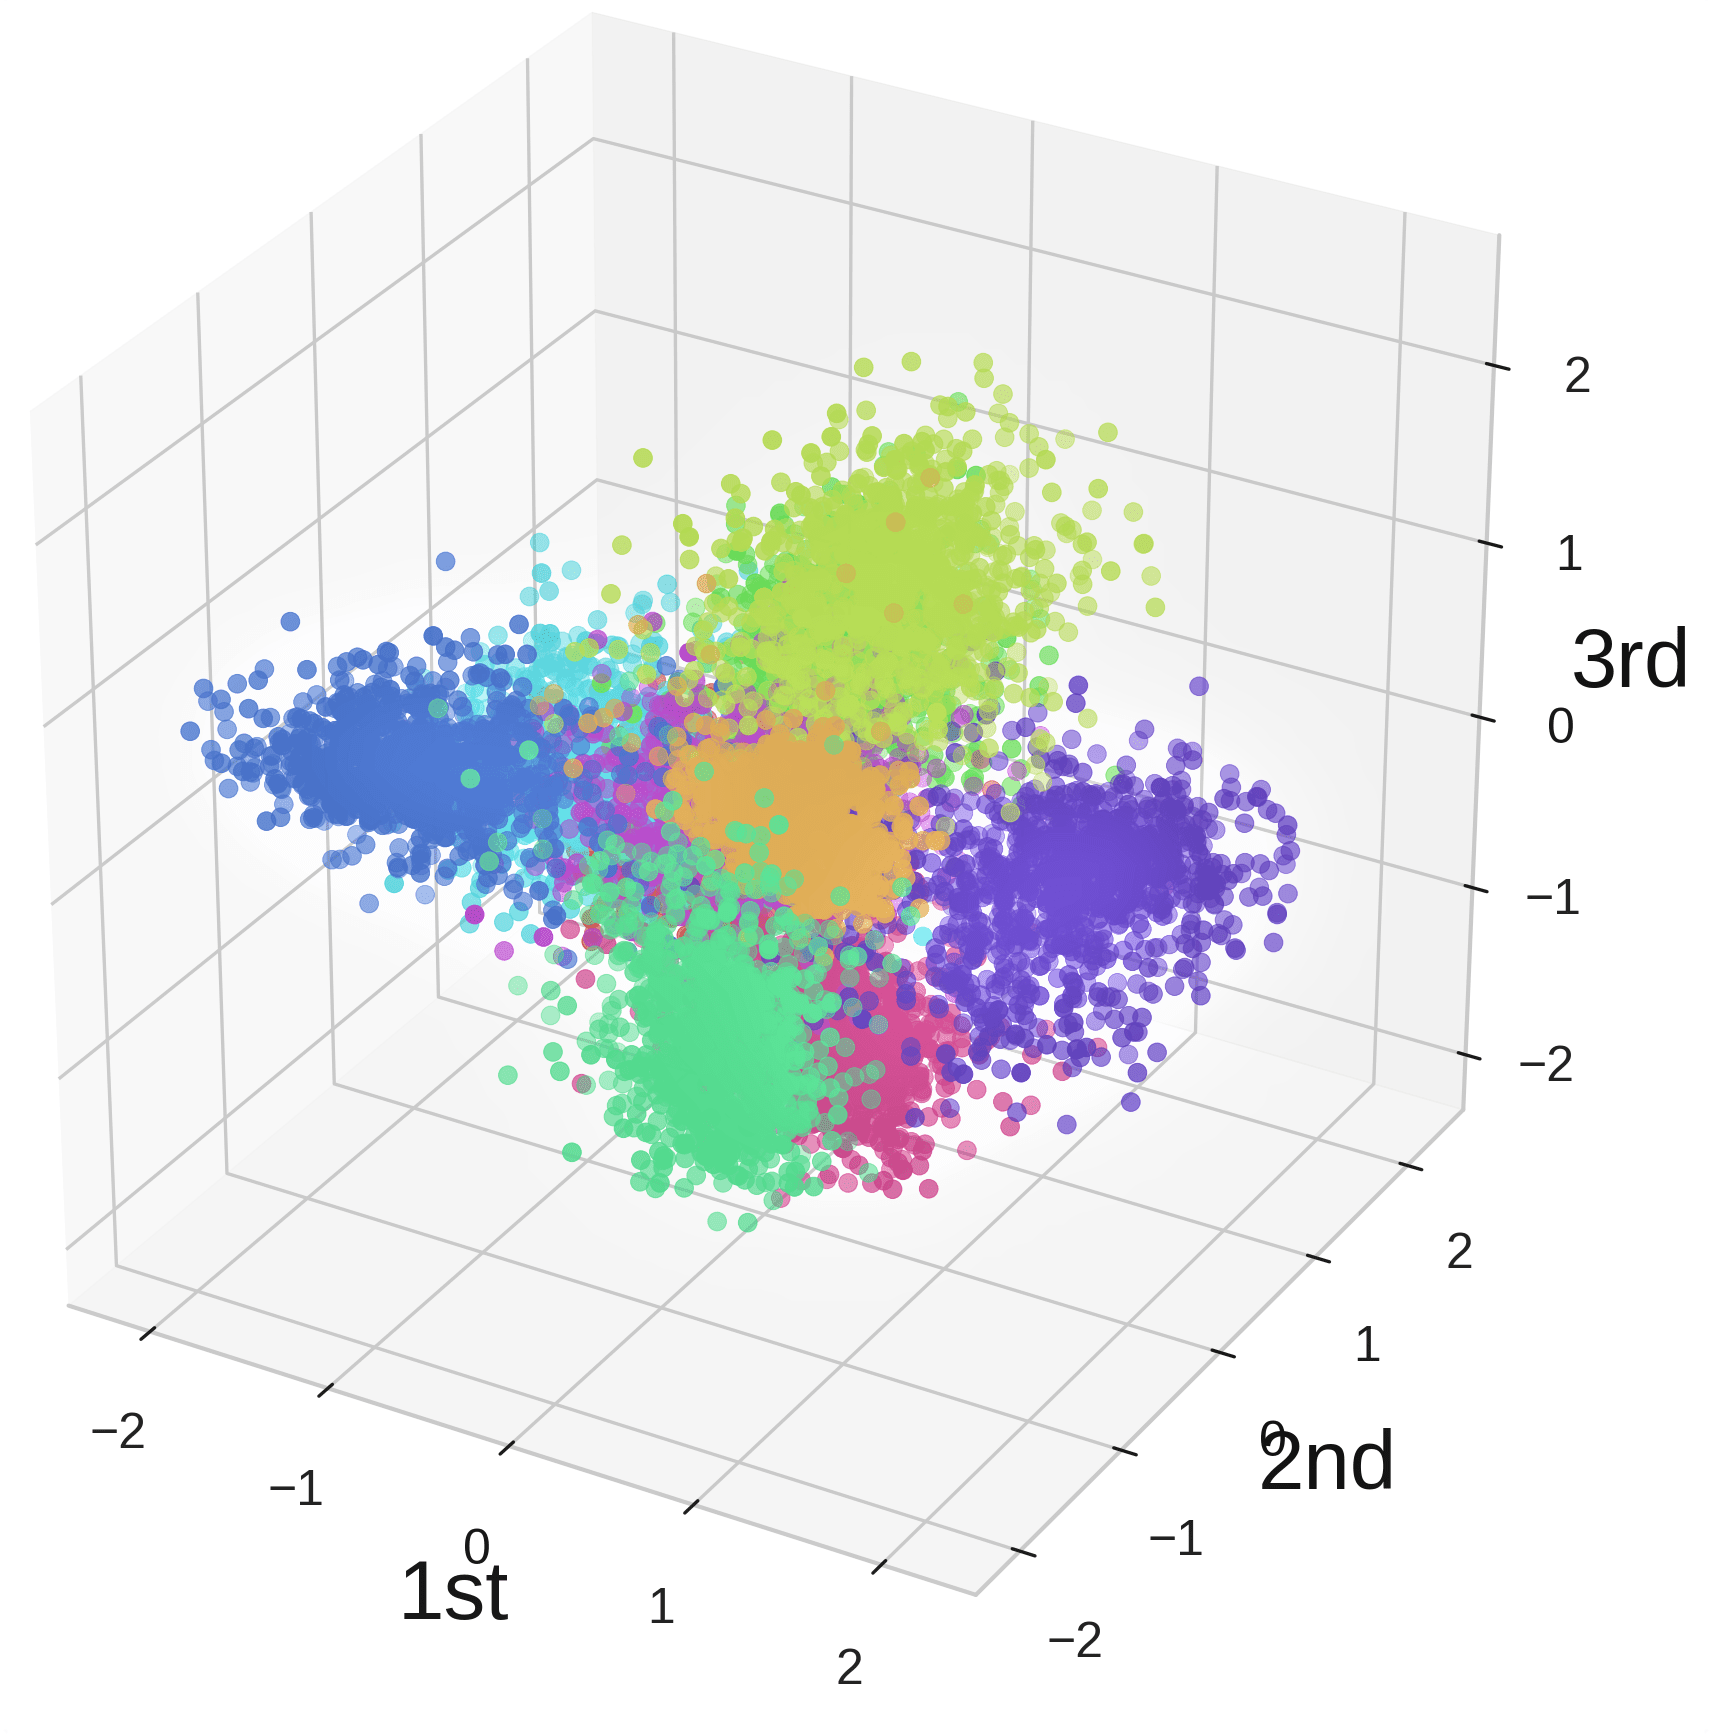
\includegraphics[width=4.1cm]{none_fc5a.png} }} 
    
    \subfloat[L1W (Before ReLU)]{{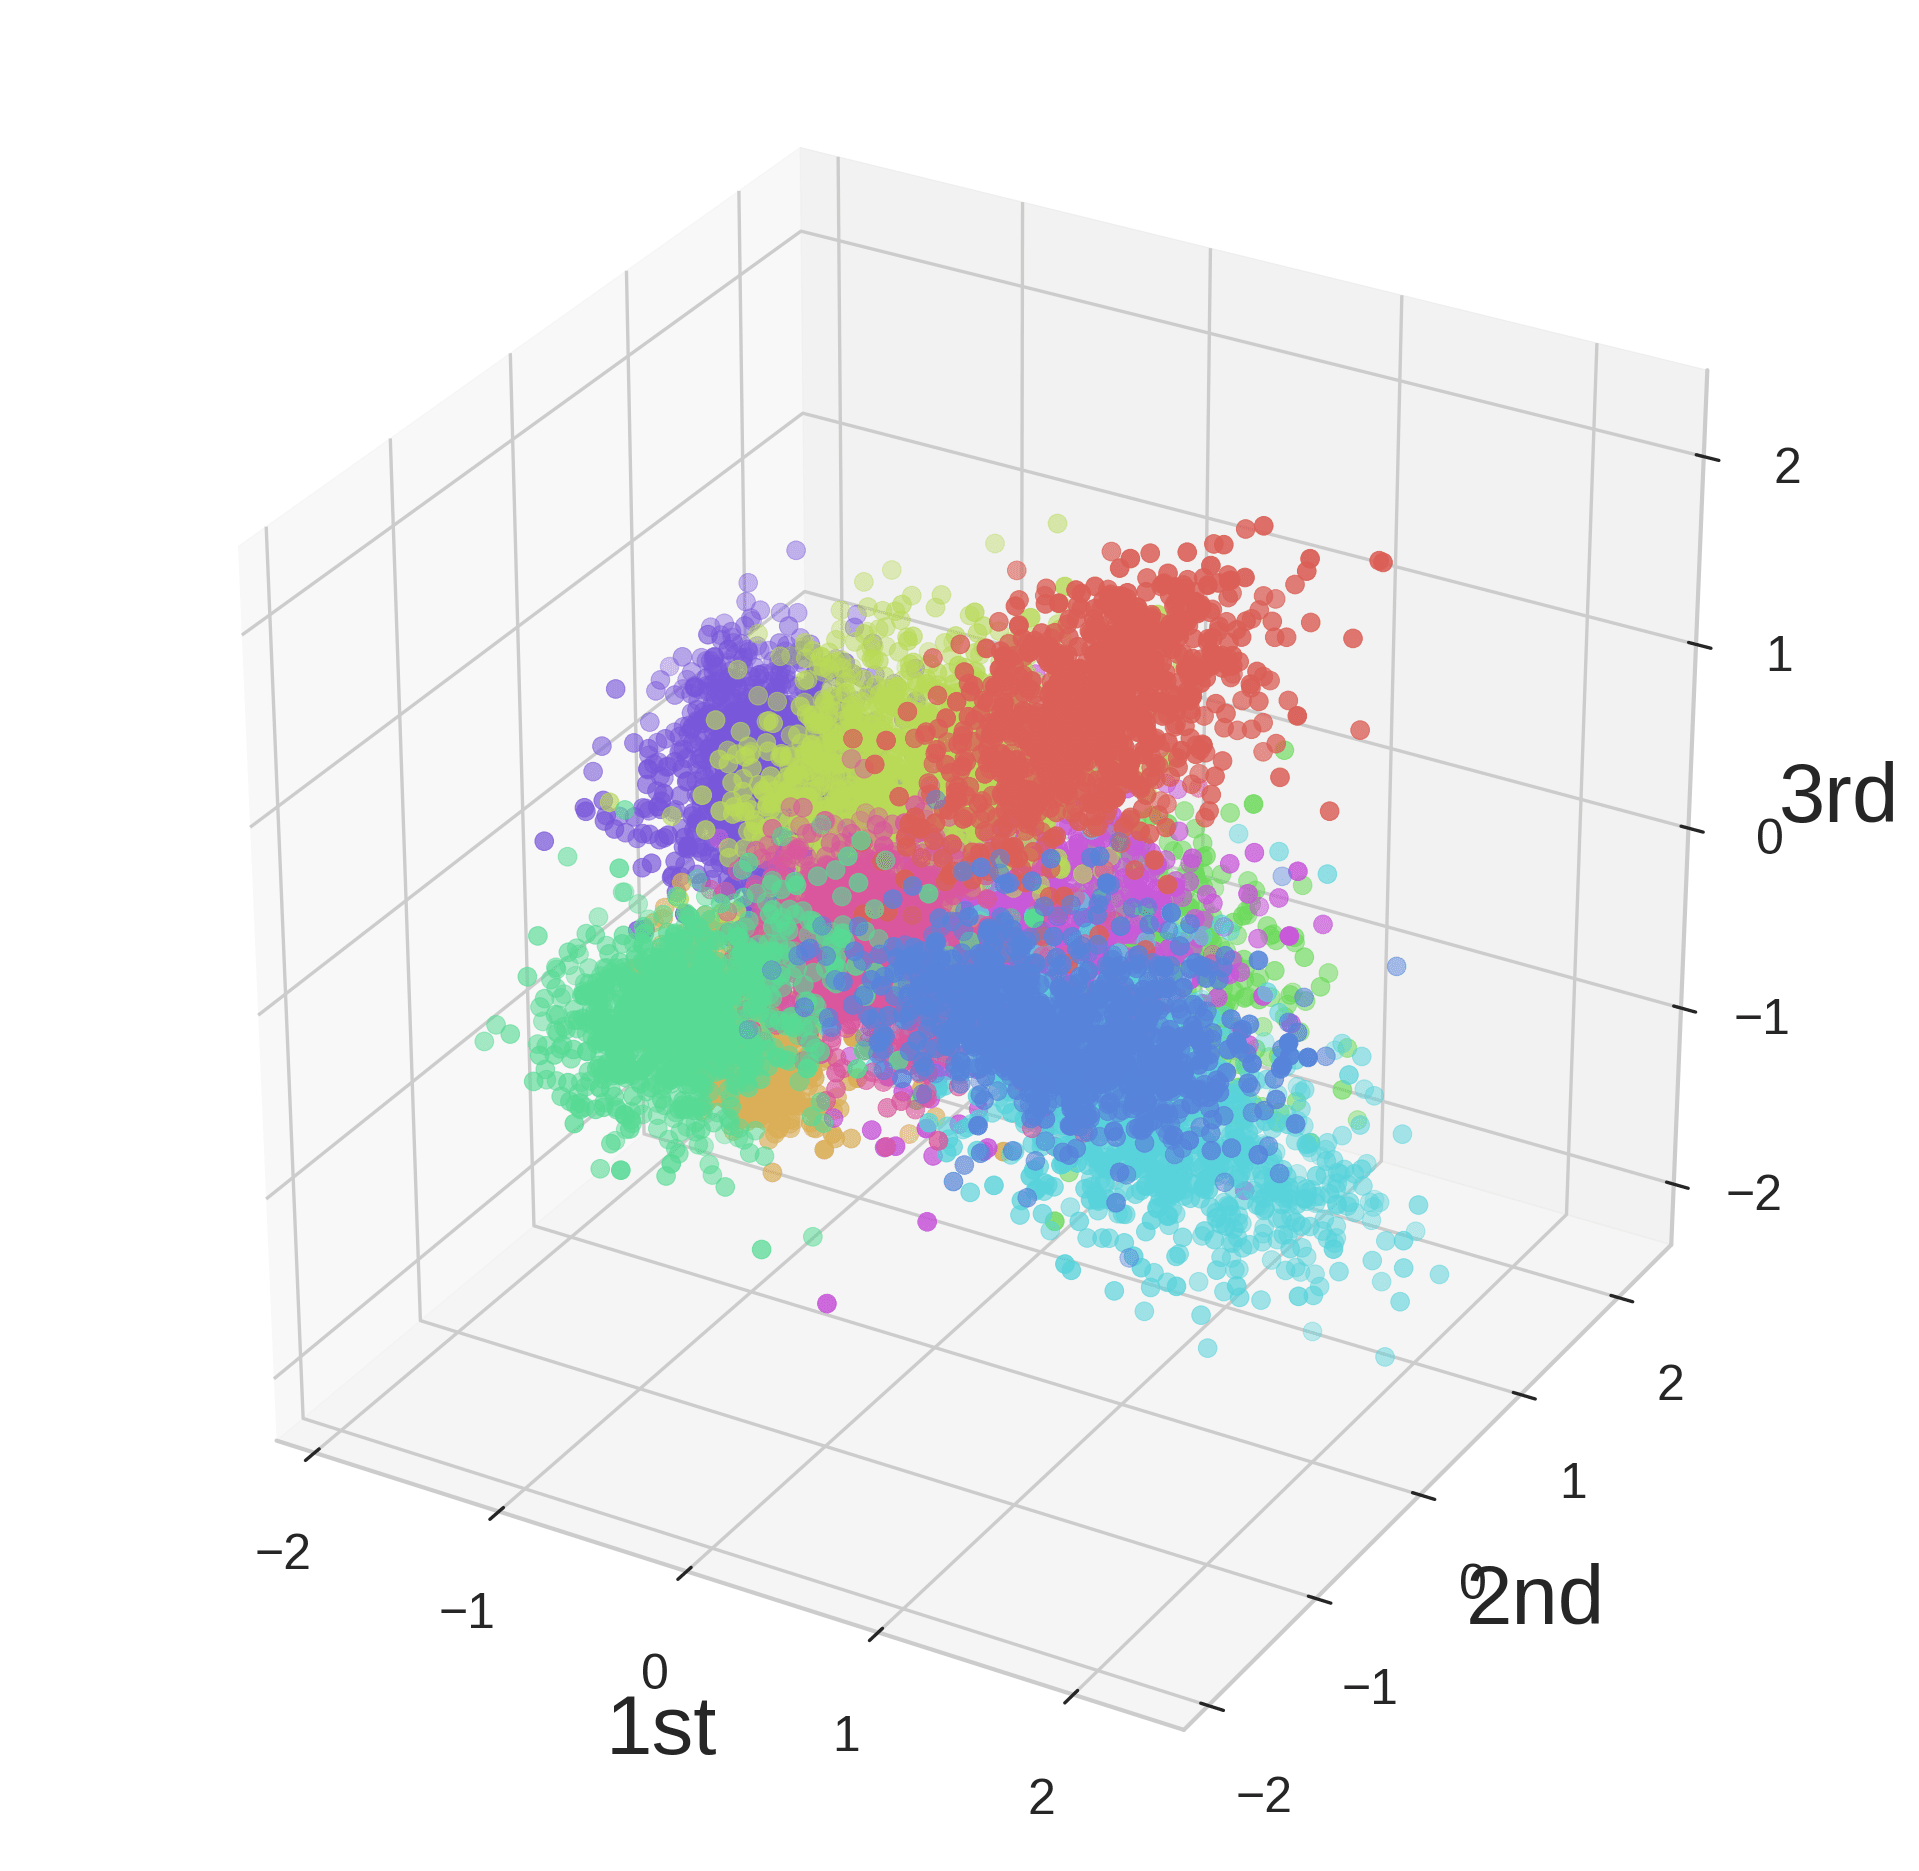
\includegraphics[width=4.5cm]{l1w_fc5.png} }}%
    \qquad\qquad\qquad
    \subfloat[L1W (After ReLU)]{{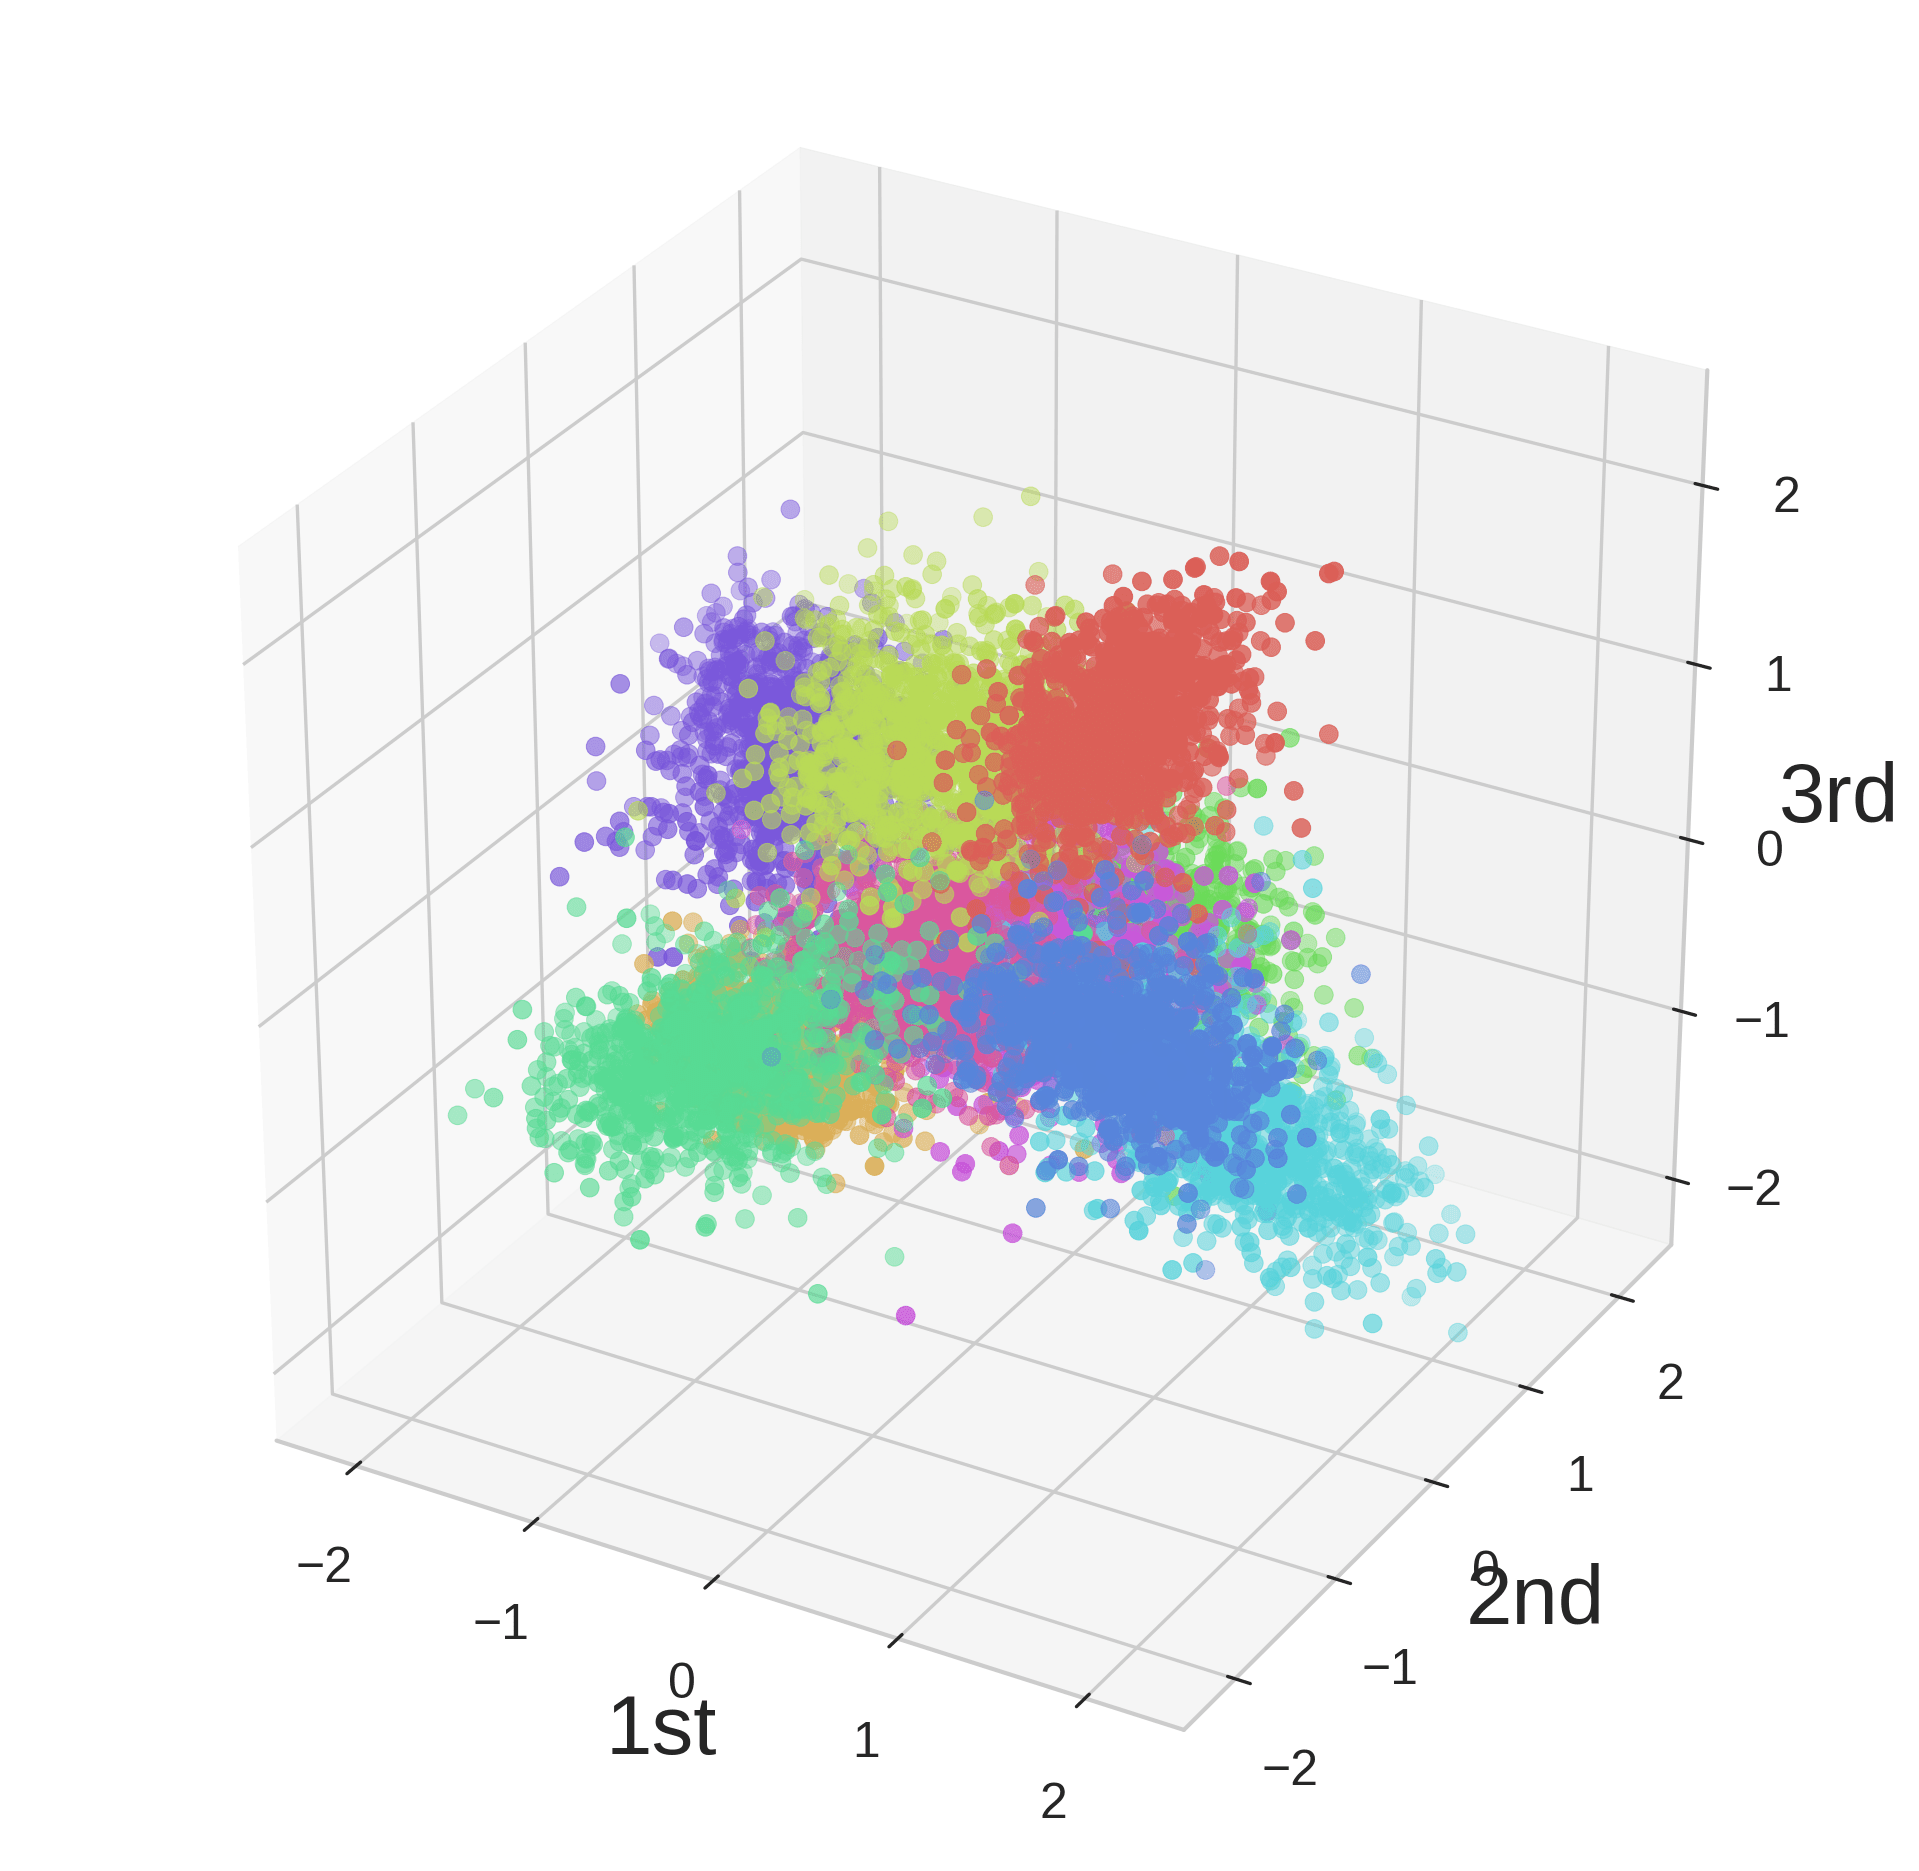
\includegraphics[width=4.5cm]{l1w_fc5a.png} }} 
    
    \subfloat[L2W (Before ReLU)]{{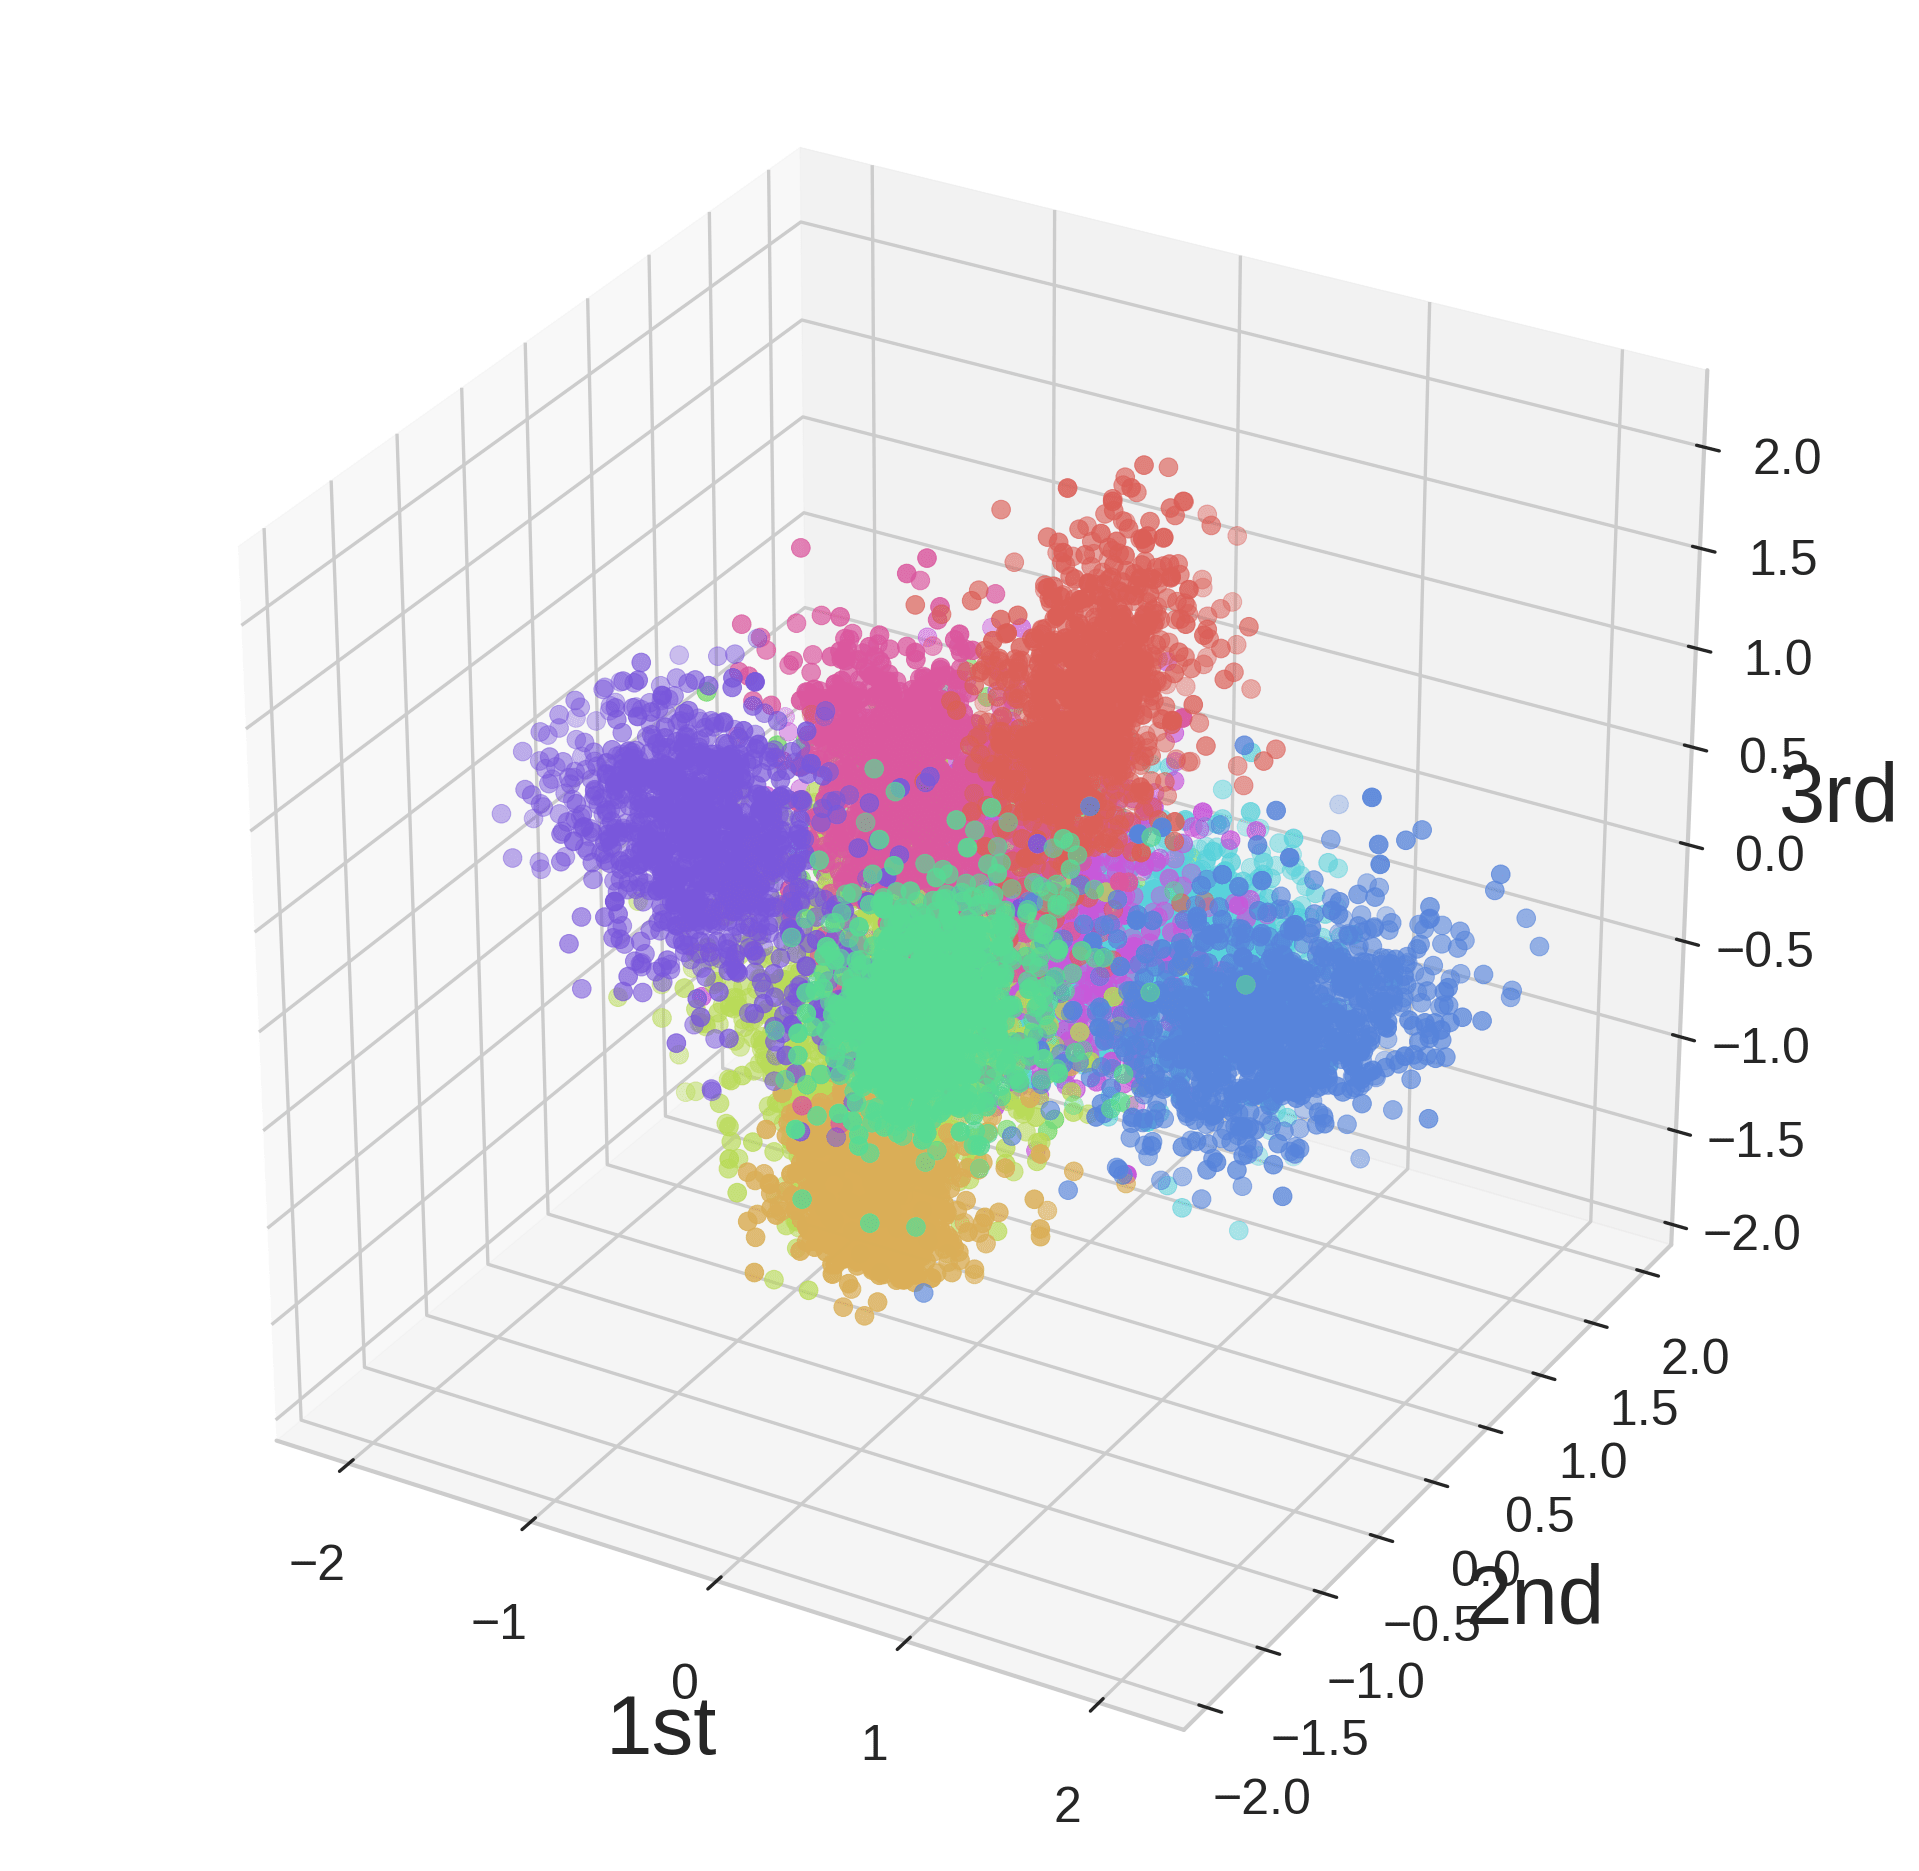
\includegraphics[width=4.5cm]{l2w_fc5.png} }}%
    \qquad\qquad\qquad
    \subfloat[L2W (After ReLU)]{{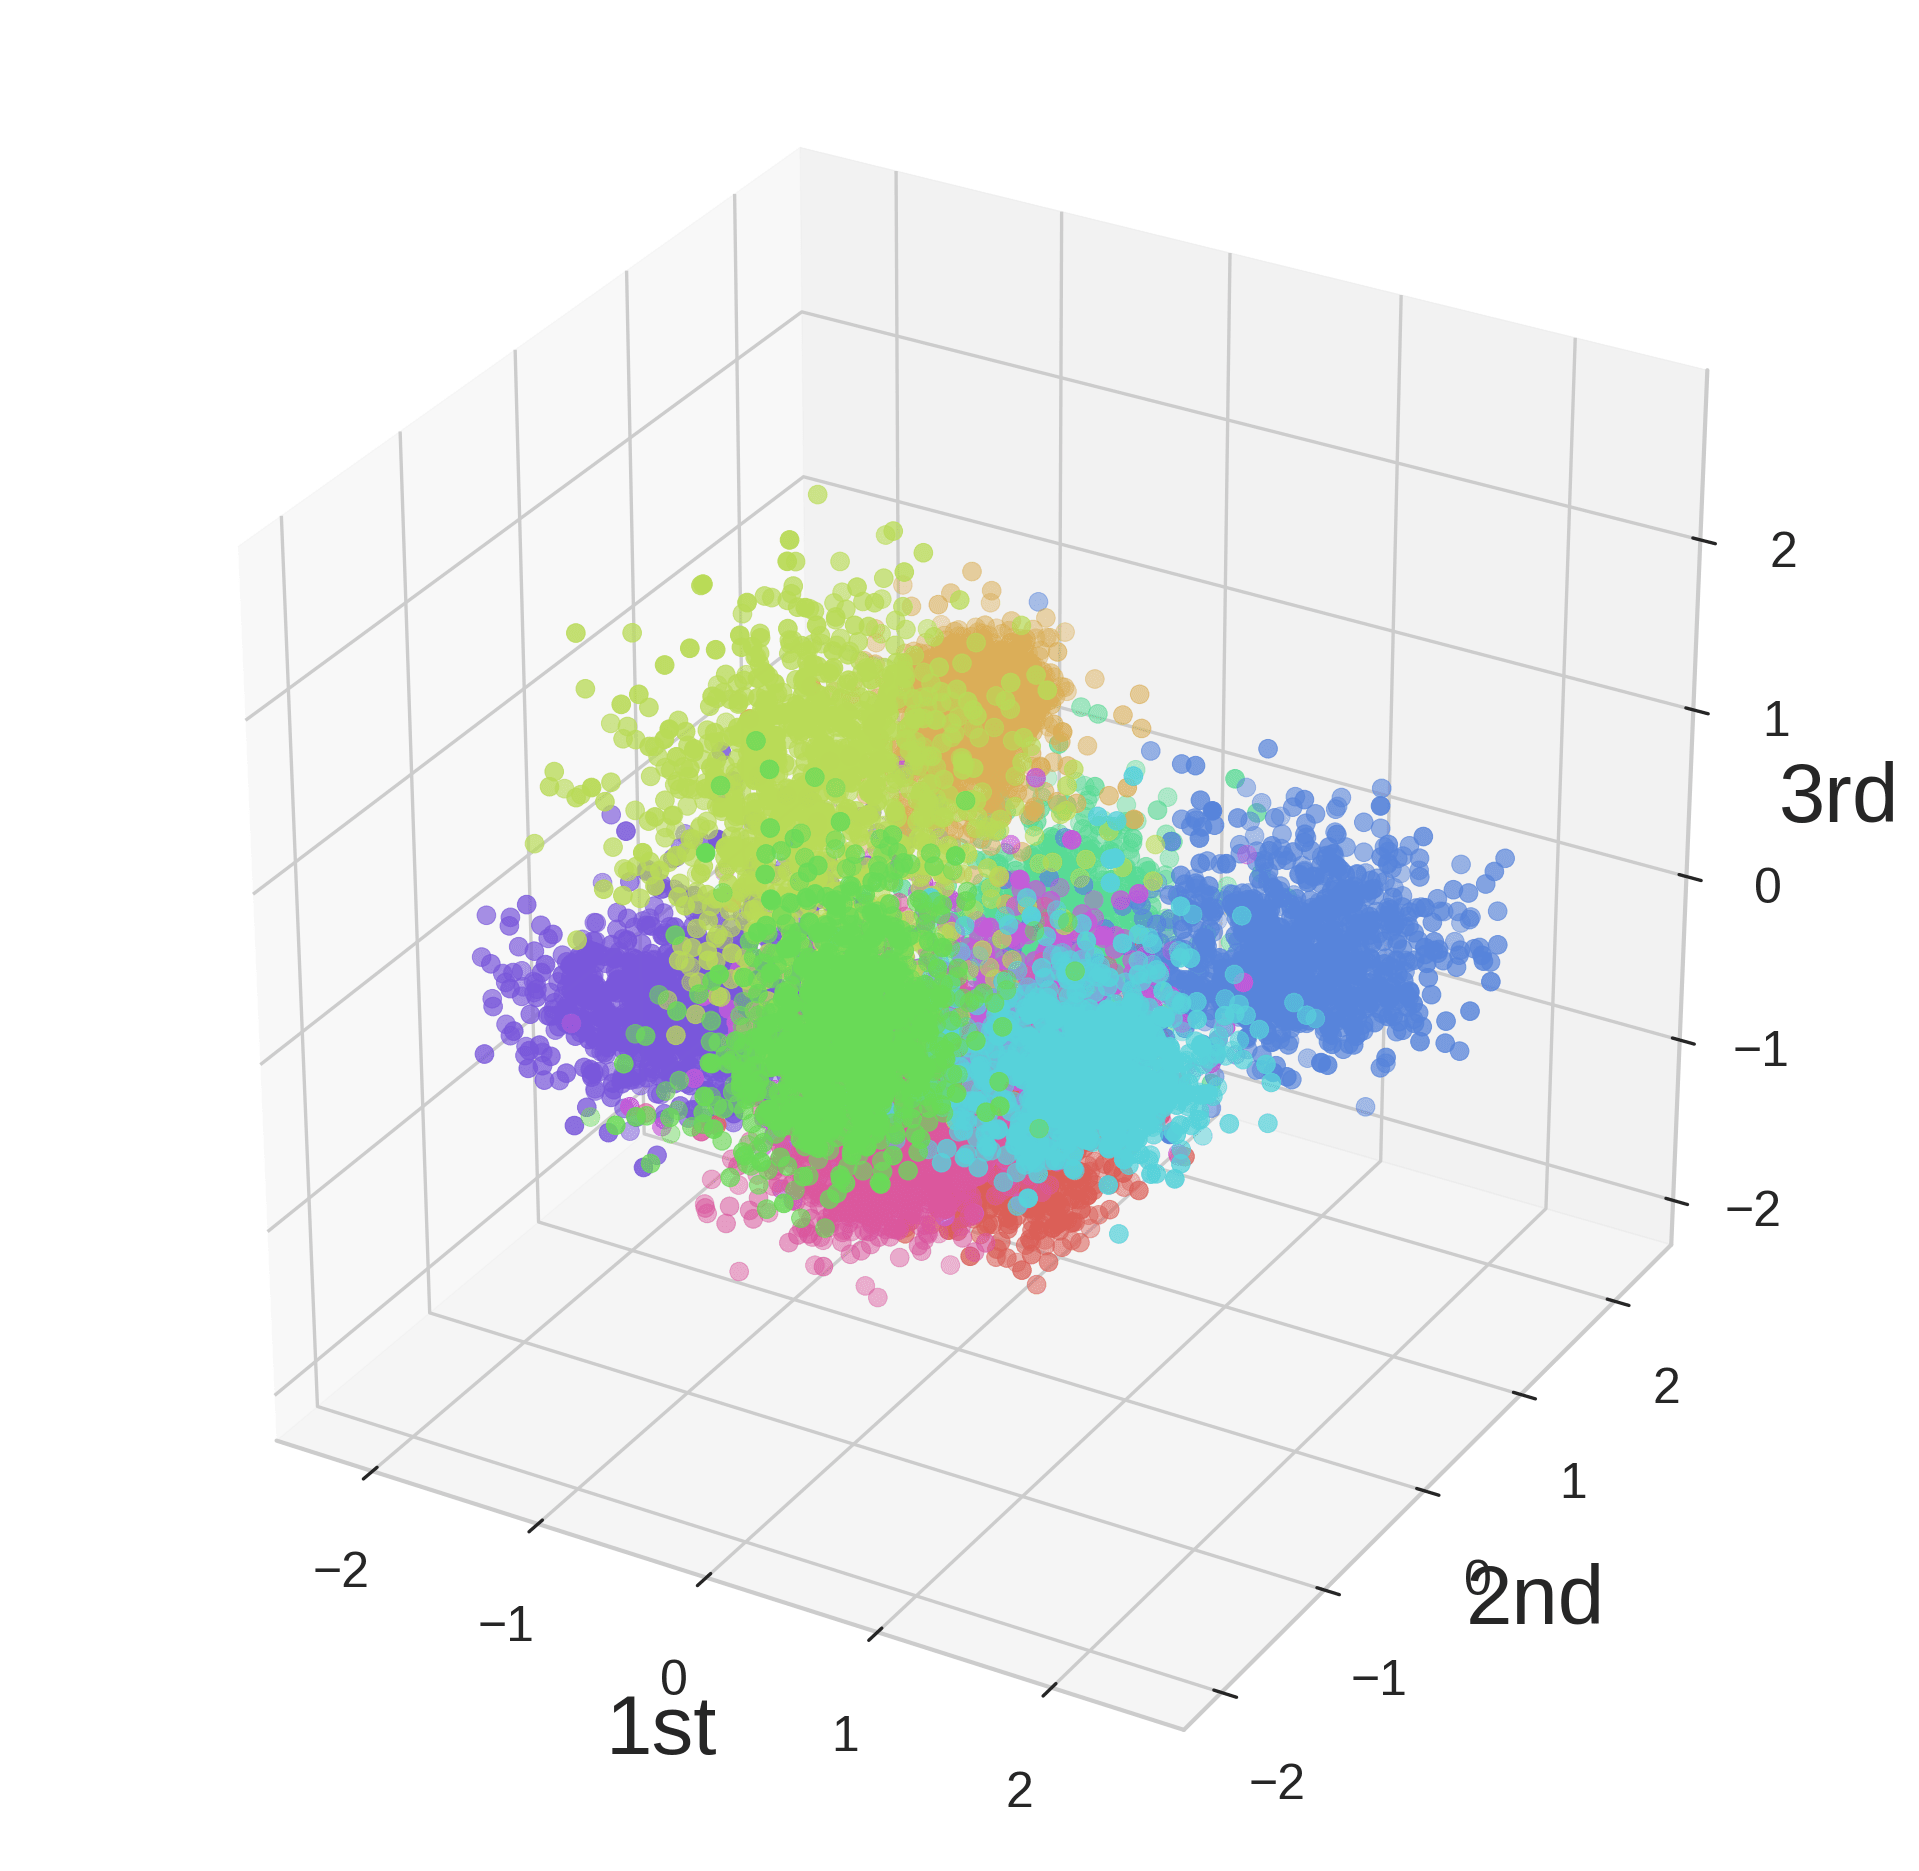
\includegraphics[width=4.5cm]{l2w_fc5a.png} }} 
     
    \captionsetup{labelformat=empty}
\caption{Figure 4: The top three principal components of learned representations (Baseline, L1W, and L2W). Note that representation characteristics of L1W and L2W are very similar to those of the baseline because weight decay methods do not directly shape representations.}%
    \label{fig:pca_1}%
\end{figure}

\begin{figure}[htbp]
% \vskip -0.6in
    \centering
    \subfloat[CR (Before ReLU)]{{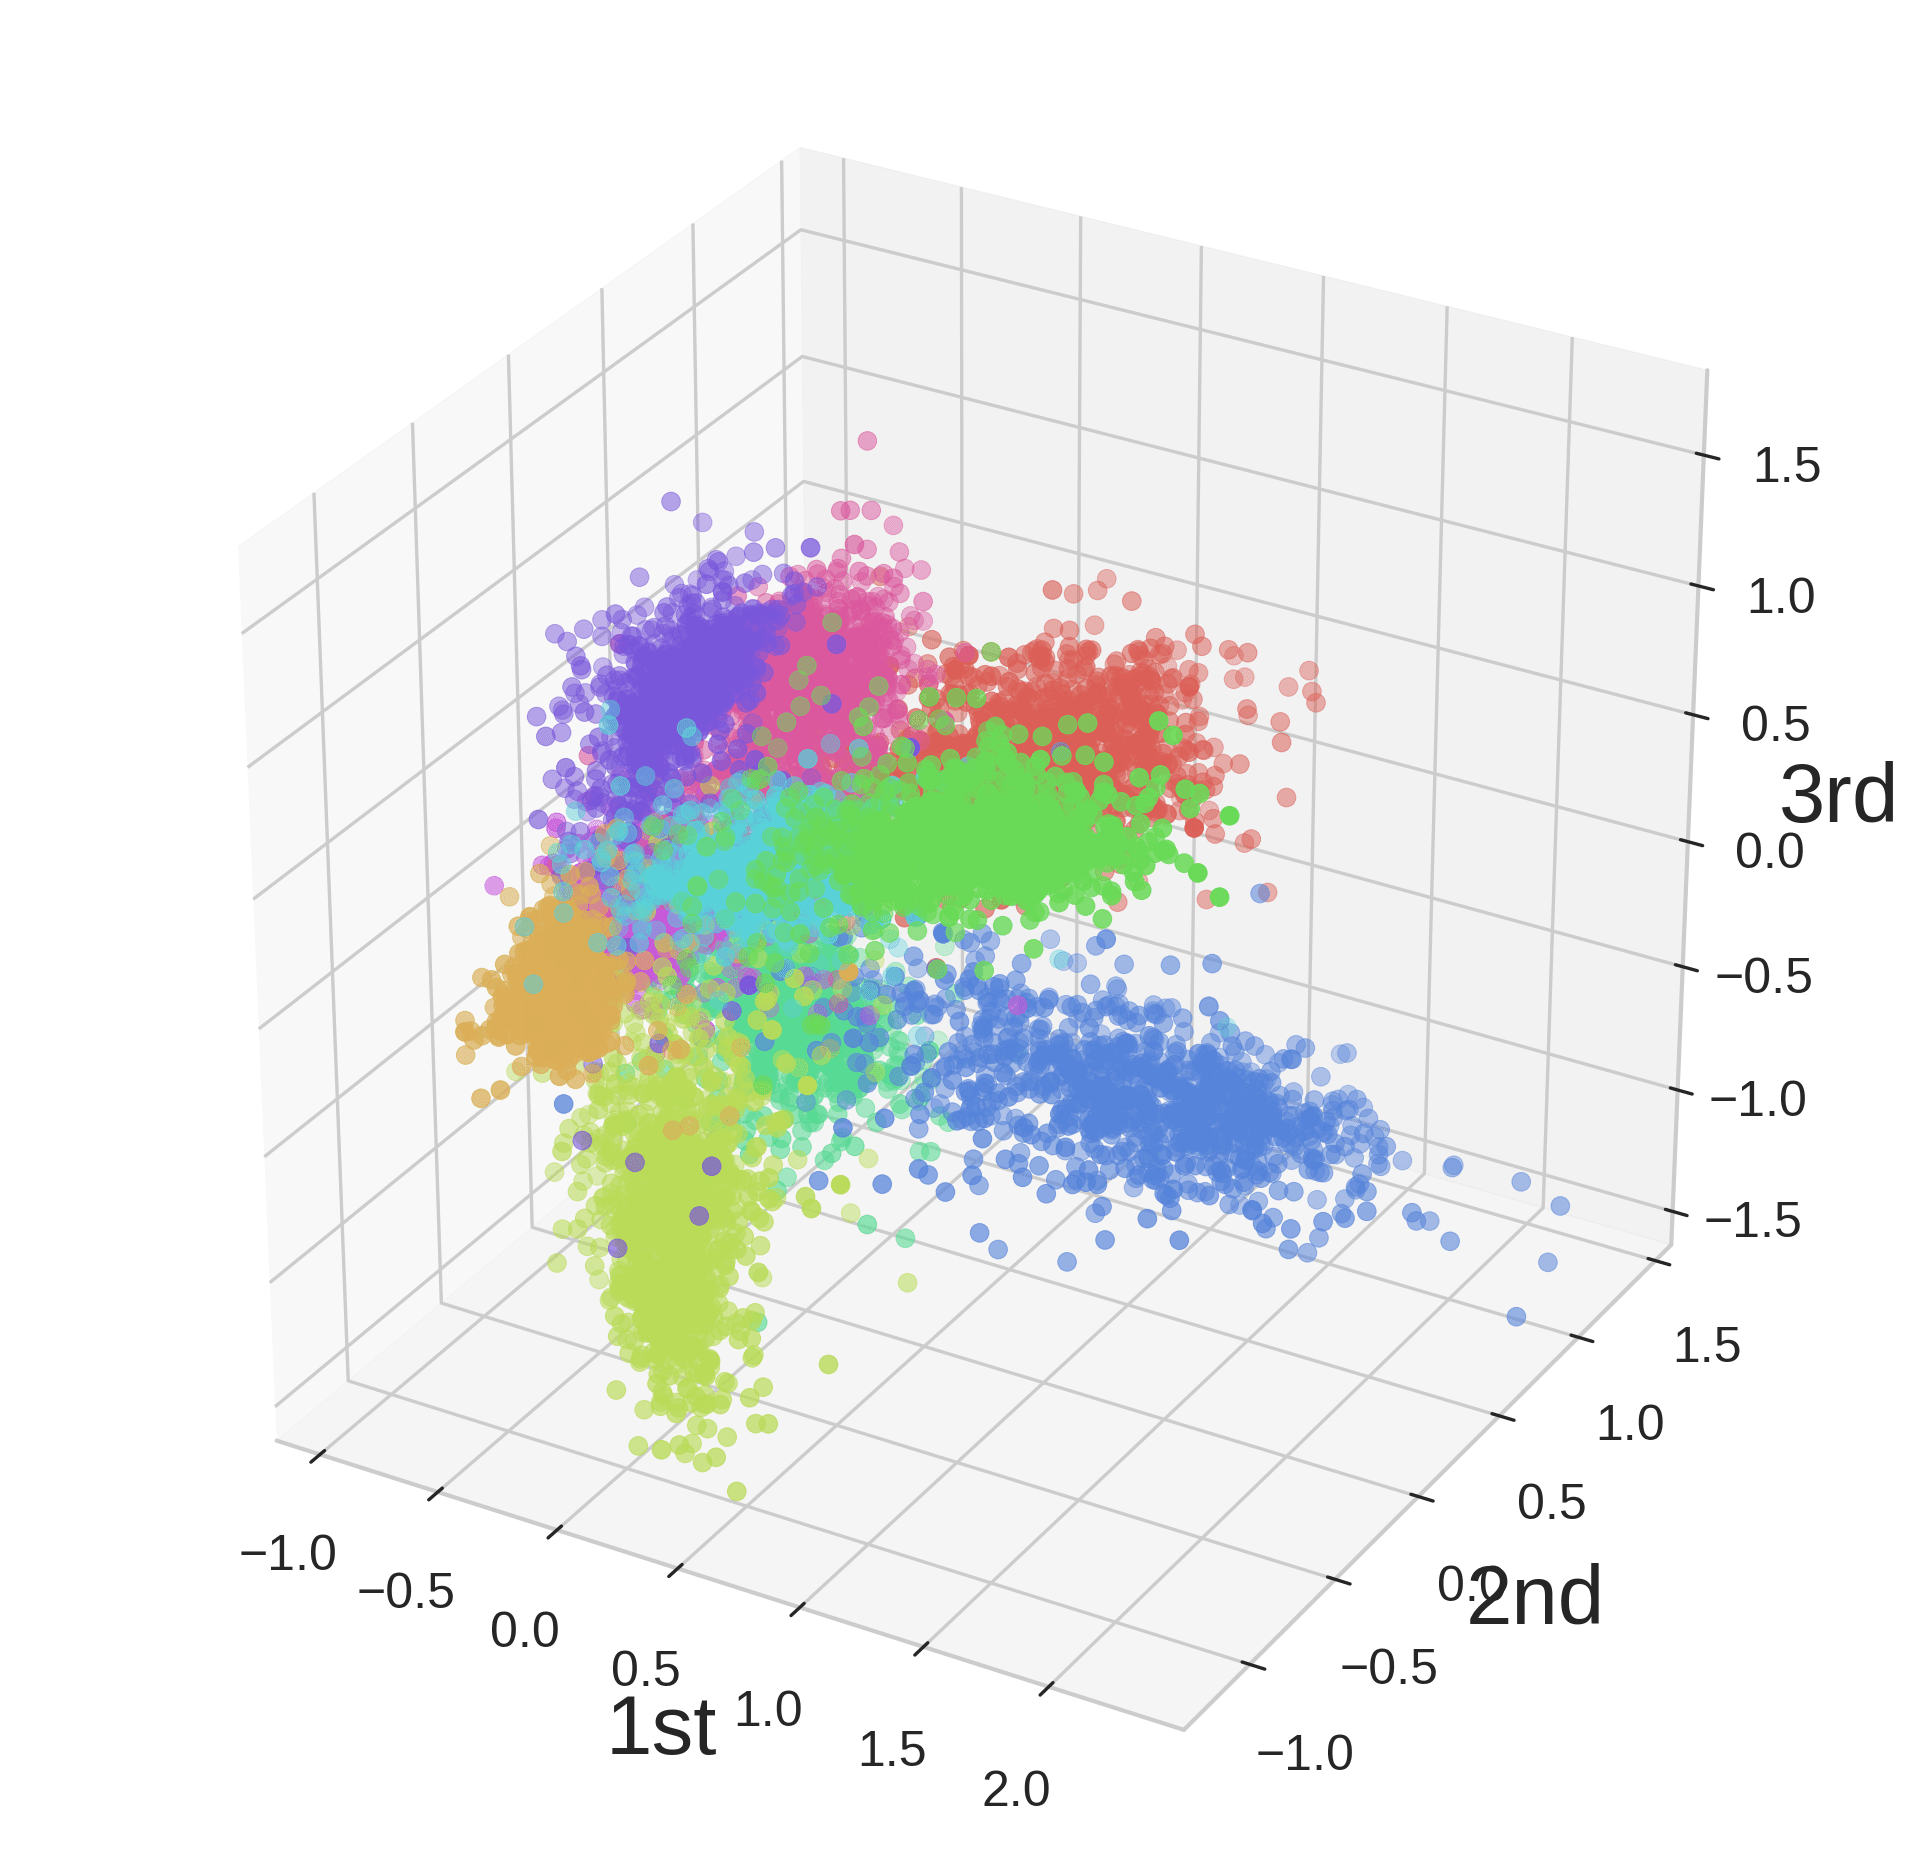
\includegraphics[width=4.5cm]{cr_fc5.png} }}%
    \qquad\qquad\qquad
    \subfloat[CR (After ReLU)]{{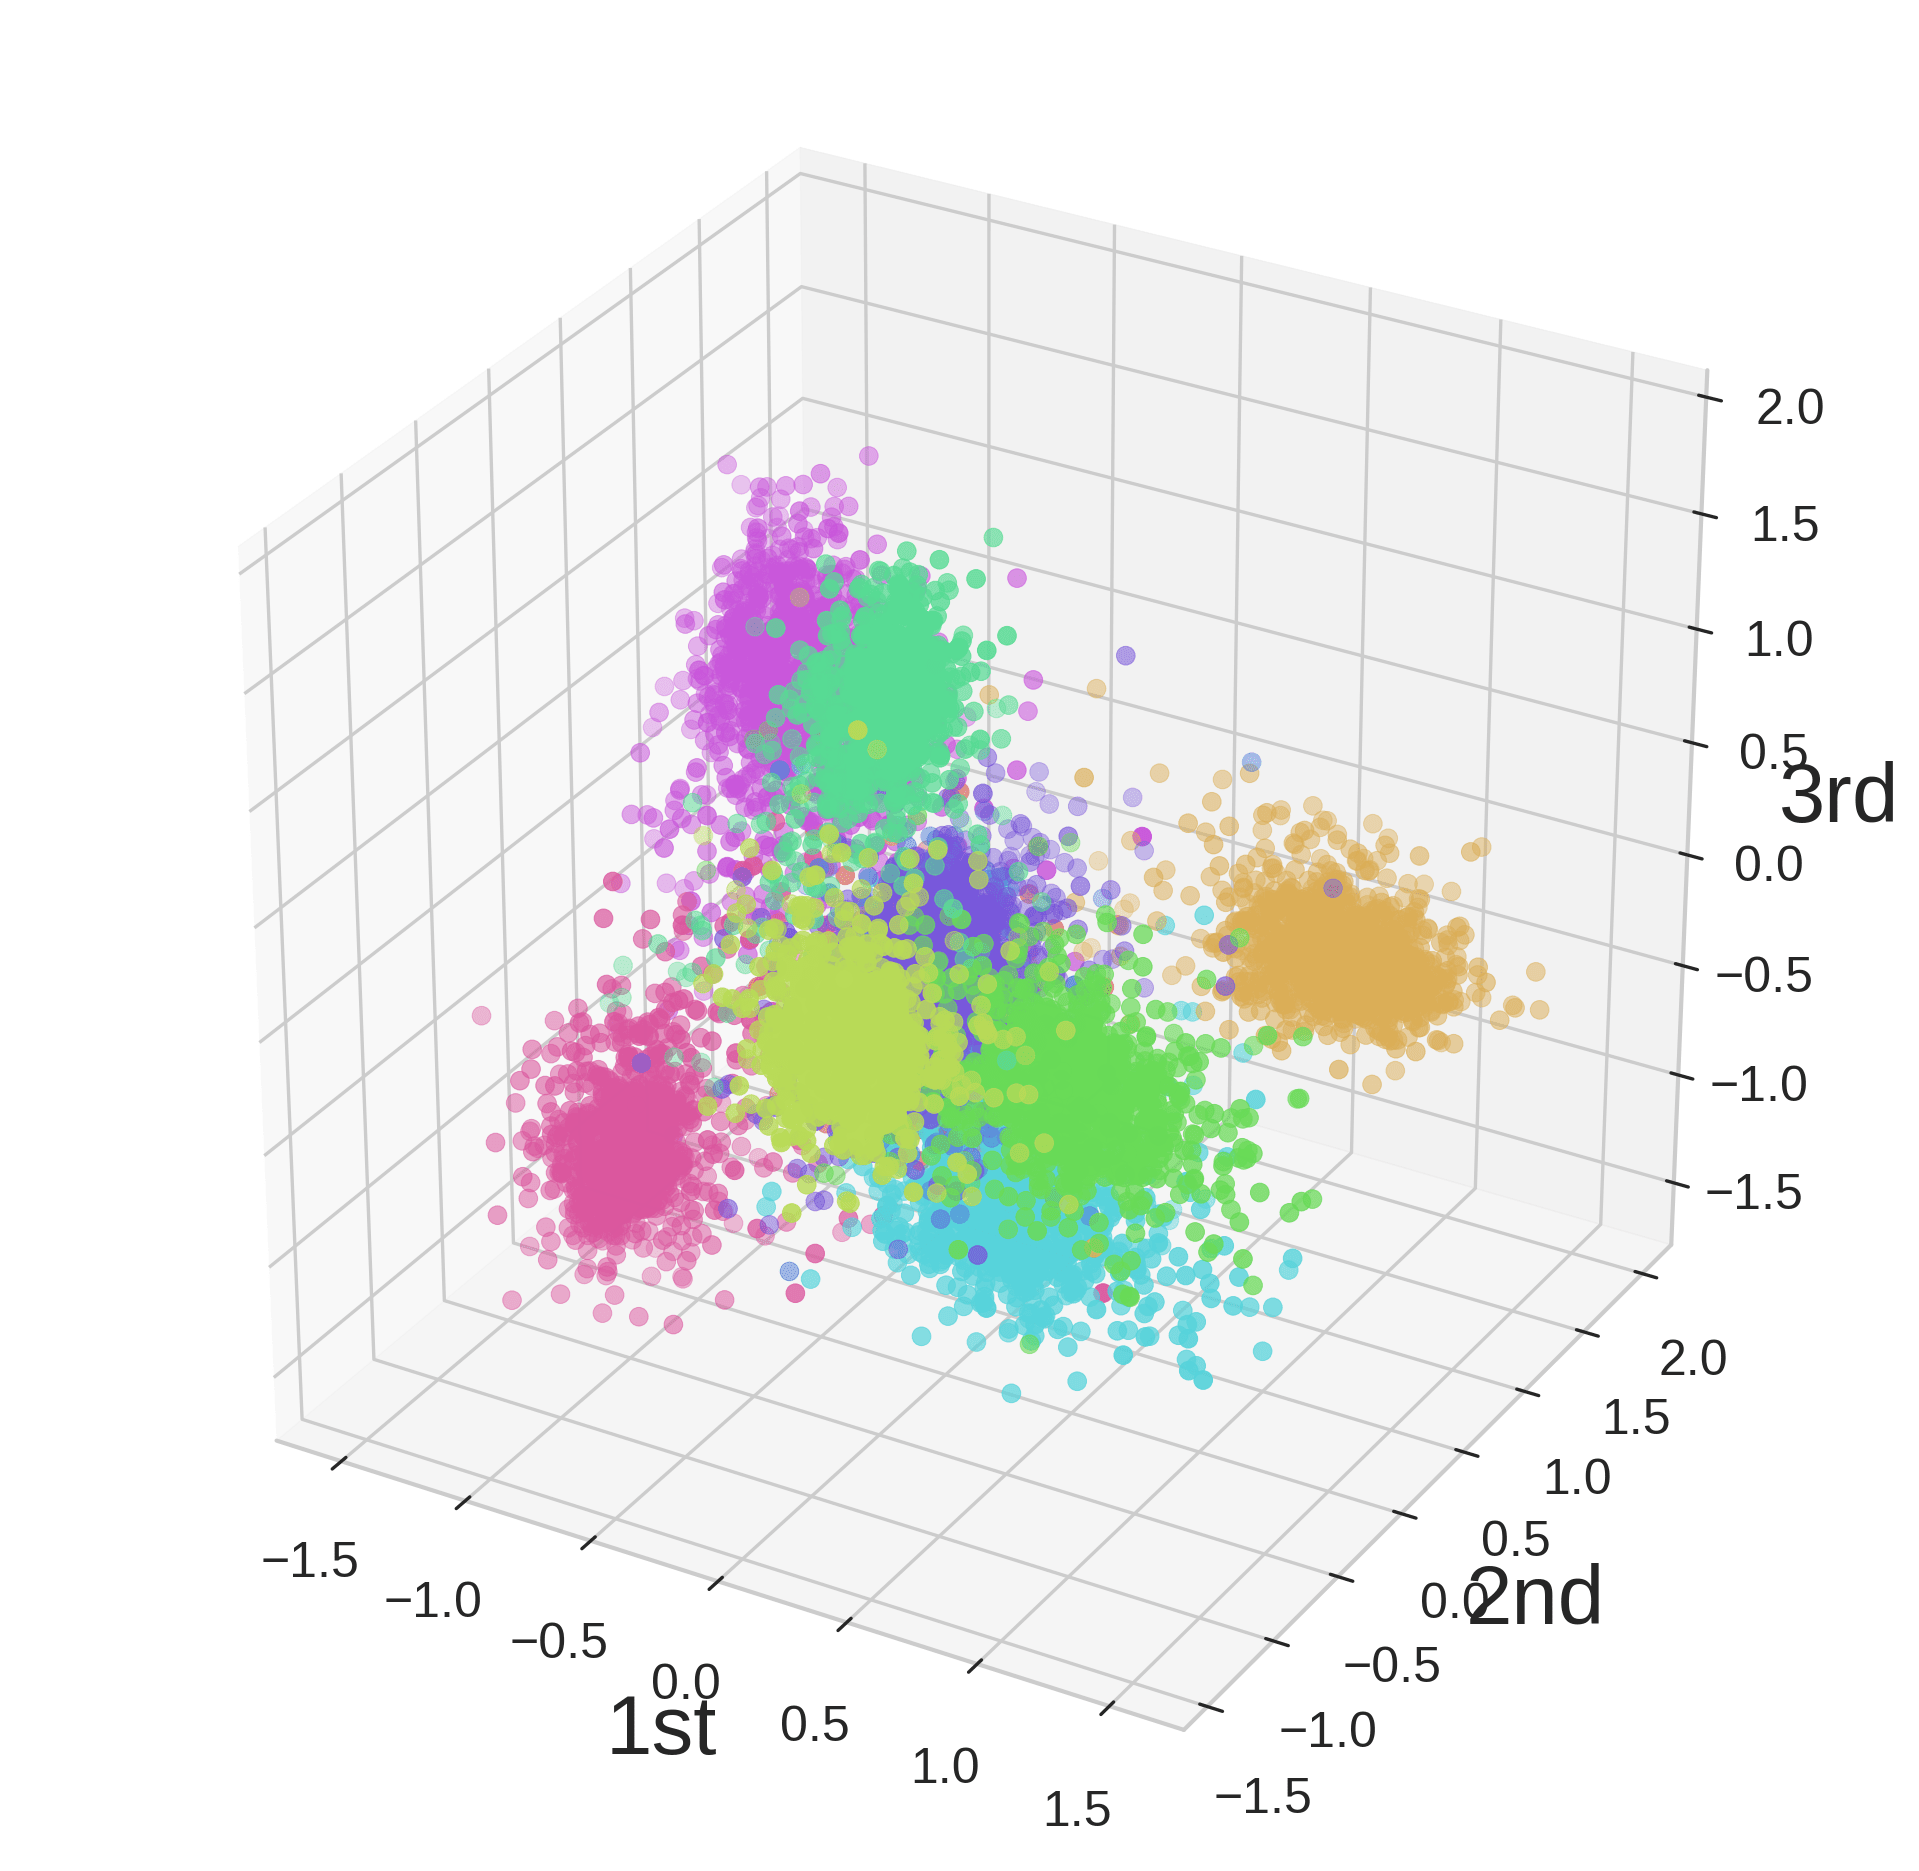
\includegraphics[width=4.5cm]{cr_fc5a.png} }}
    
    \subfloat[cw-CR (Before ReLU)]{{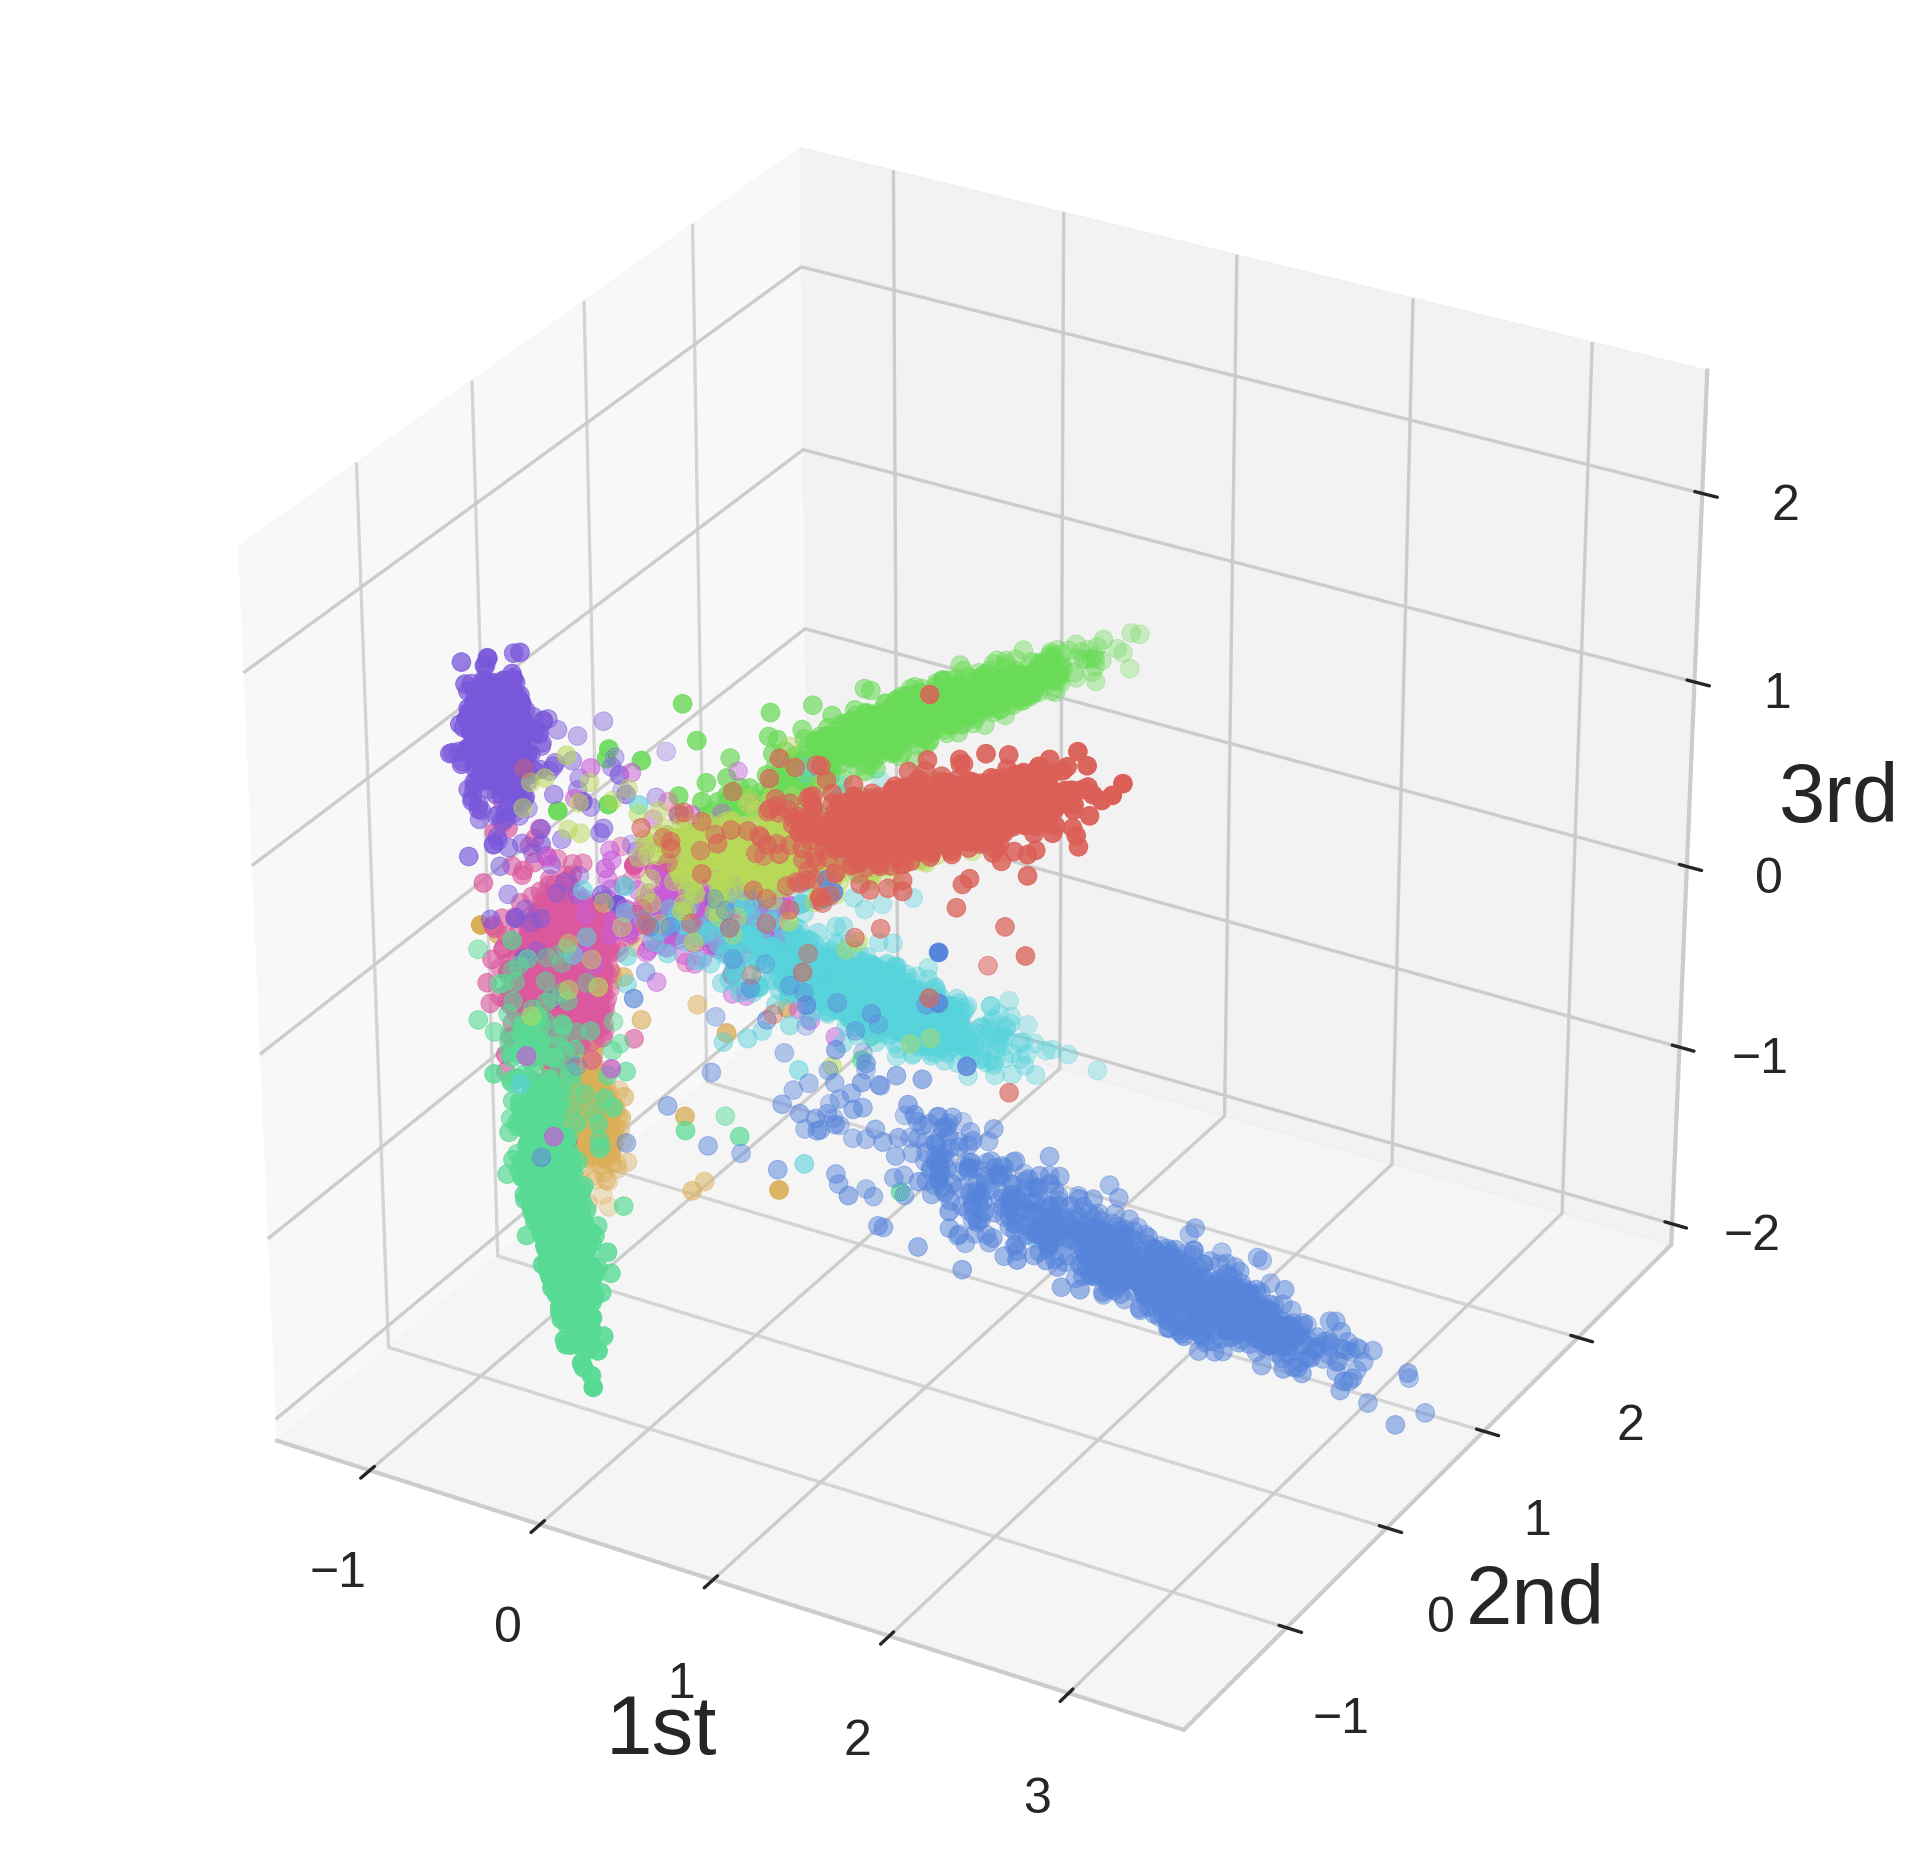
\includegraphics[width=4.5cm]{cw_cr_fc5.png} }}%
    \qquad\qquad\qquad
    \subfloat[cw-CR (After ReLU)]{{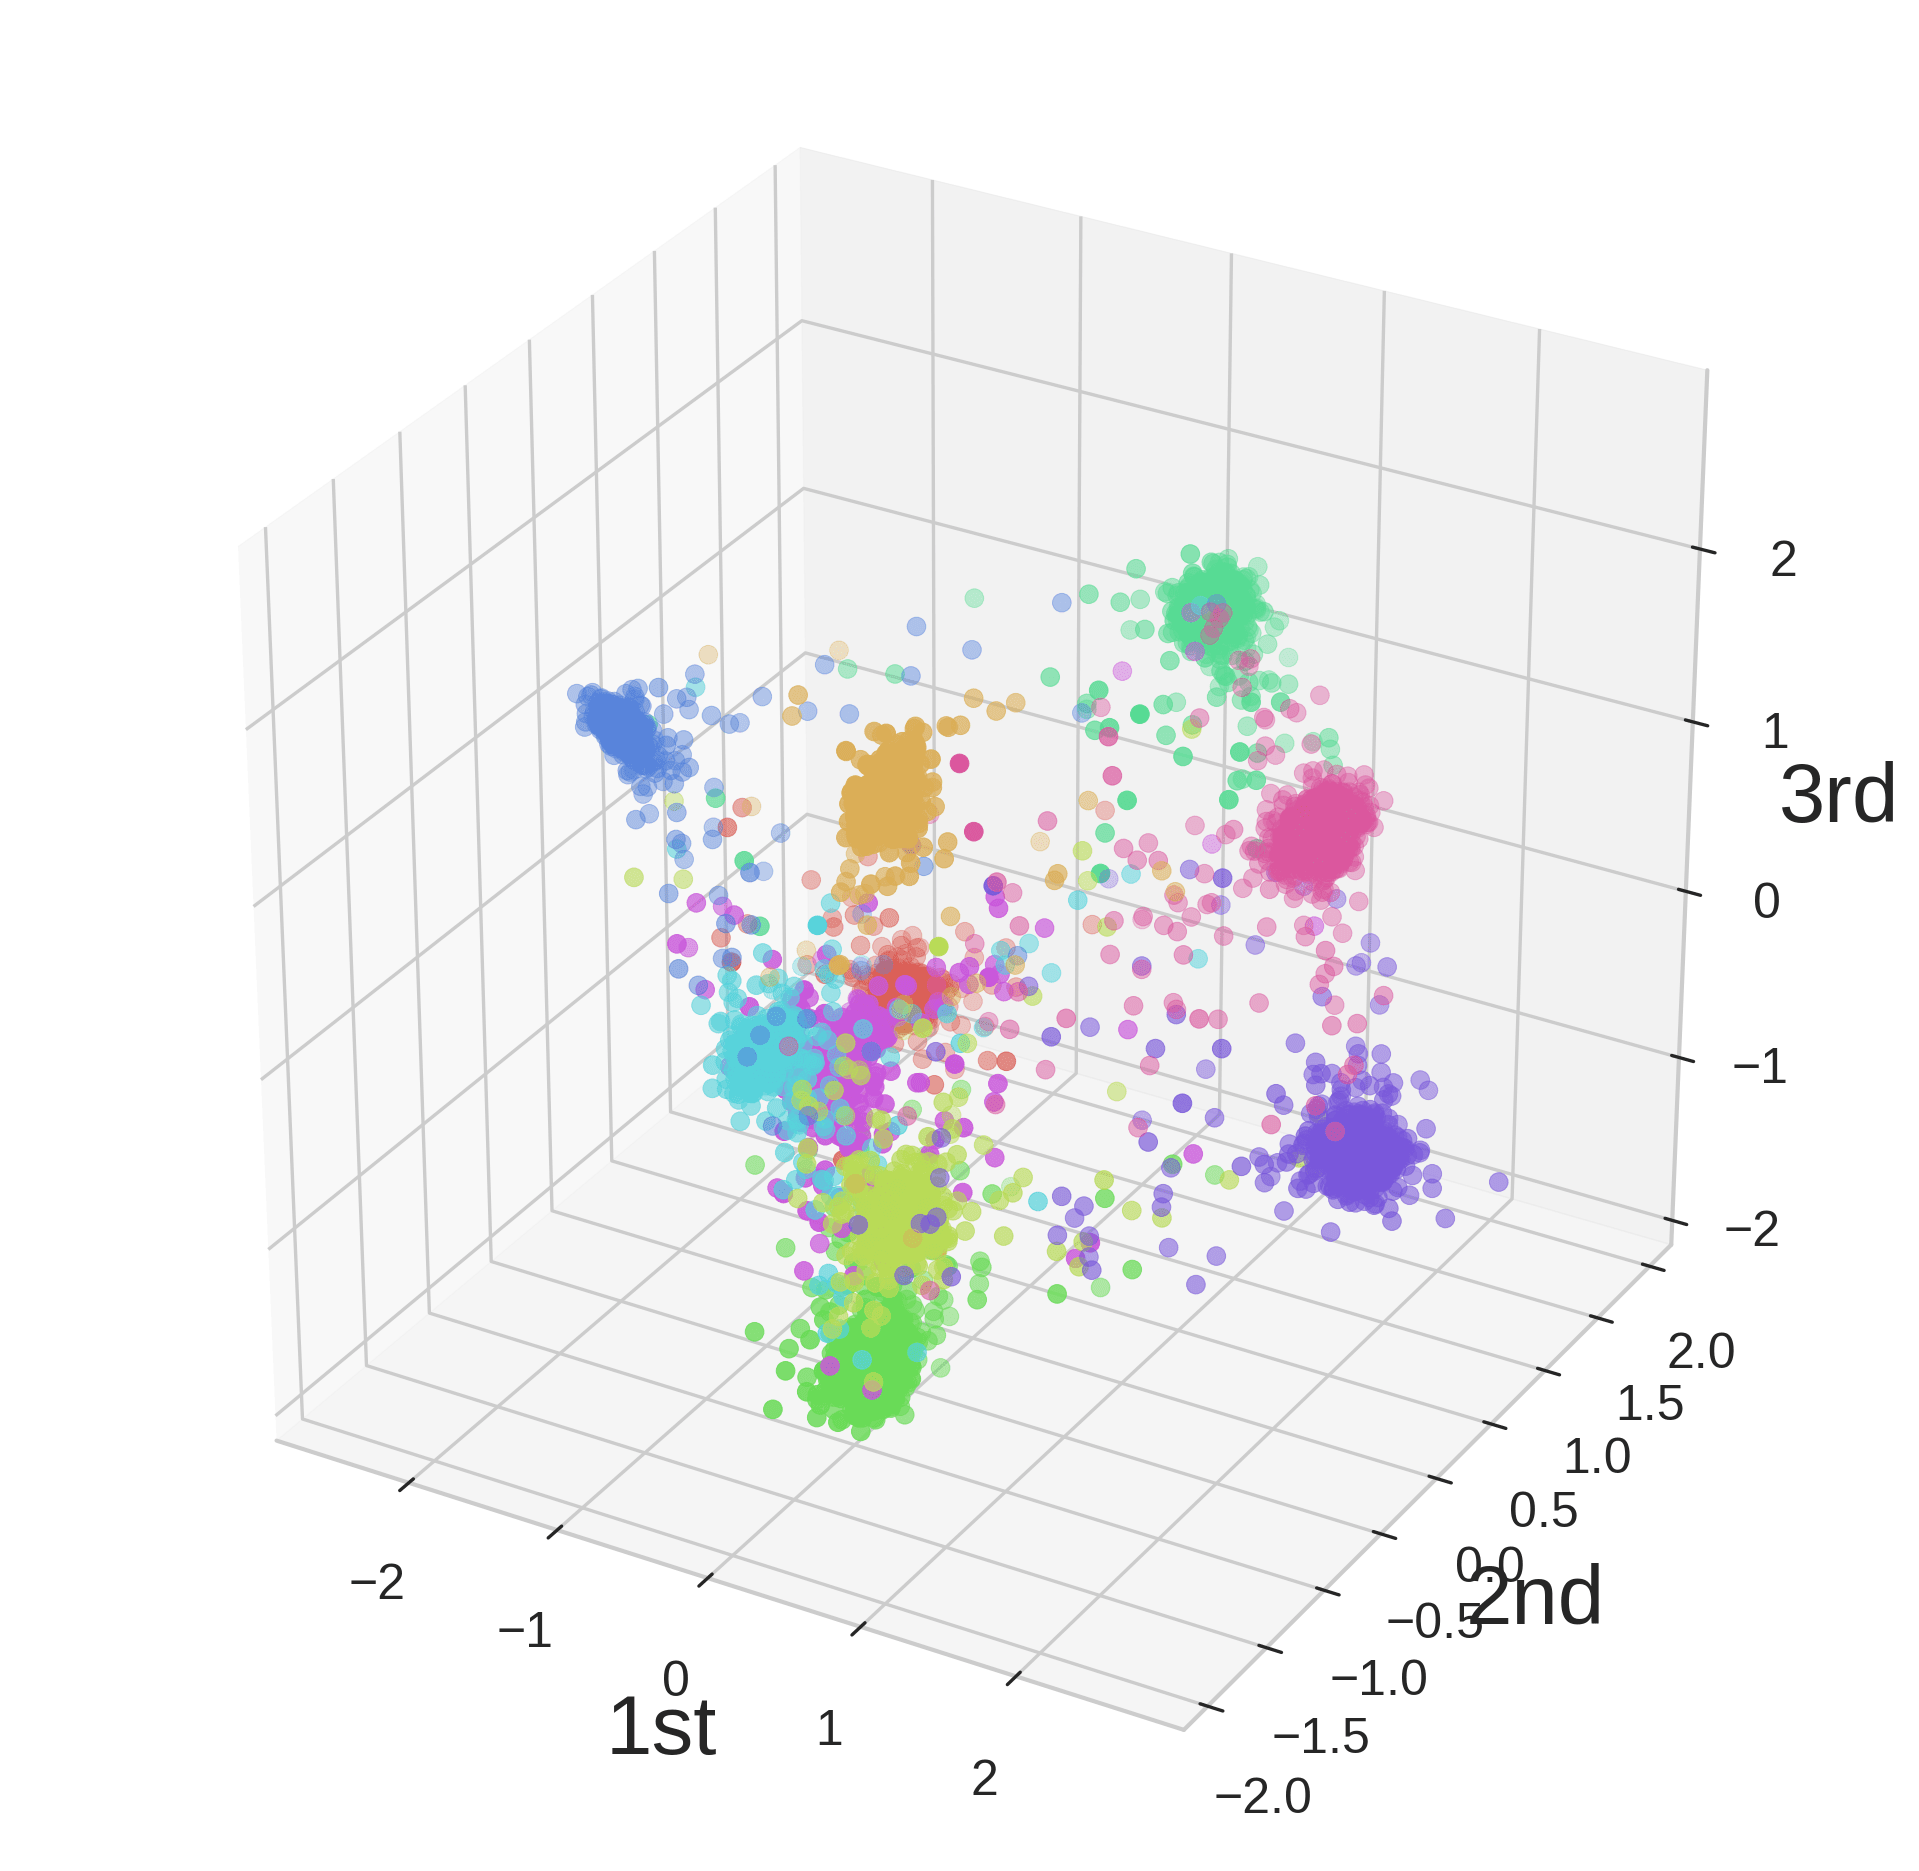
\includegraphics[width=4.5cm]{cw_cr_fc5a.png} }}
    
    \subfloat[VR (Before ReLU)]{{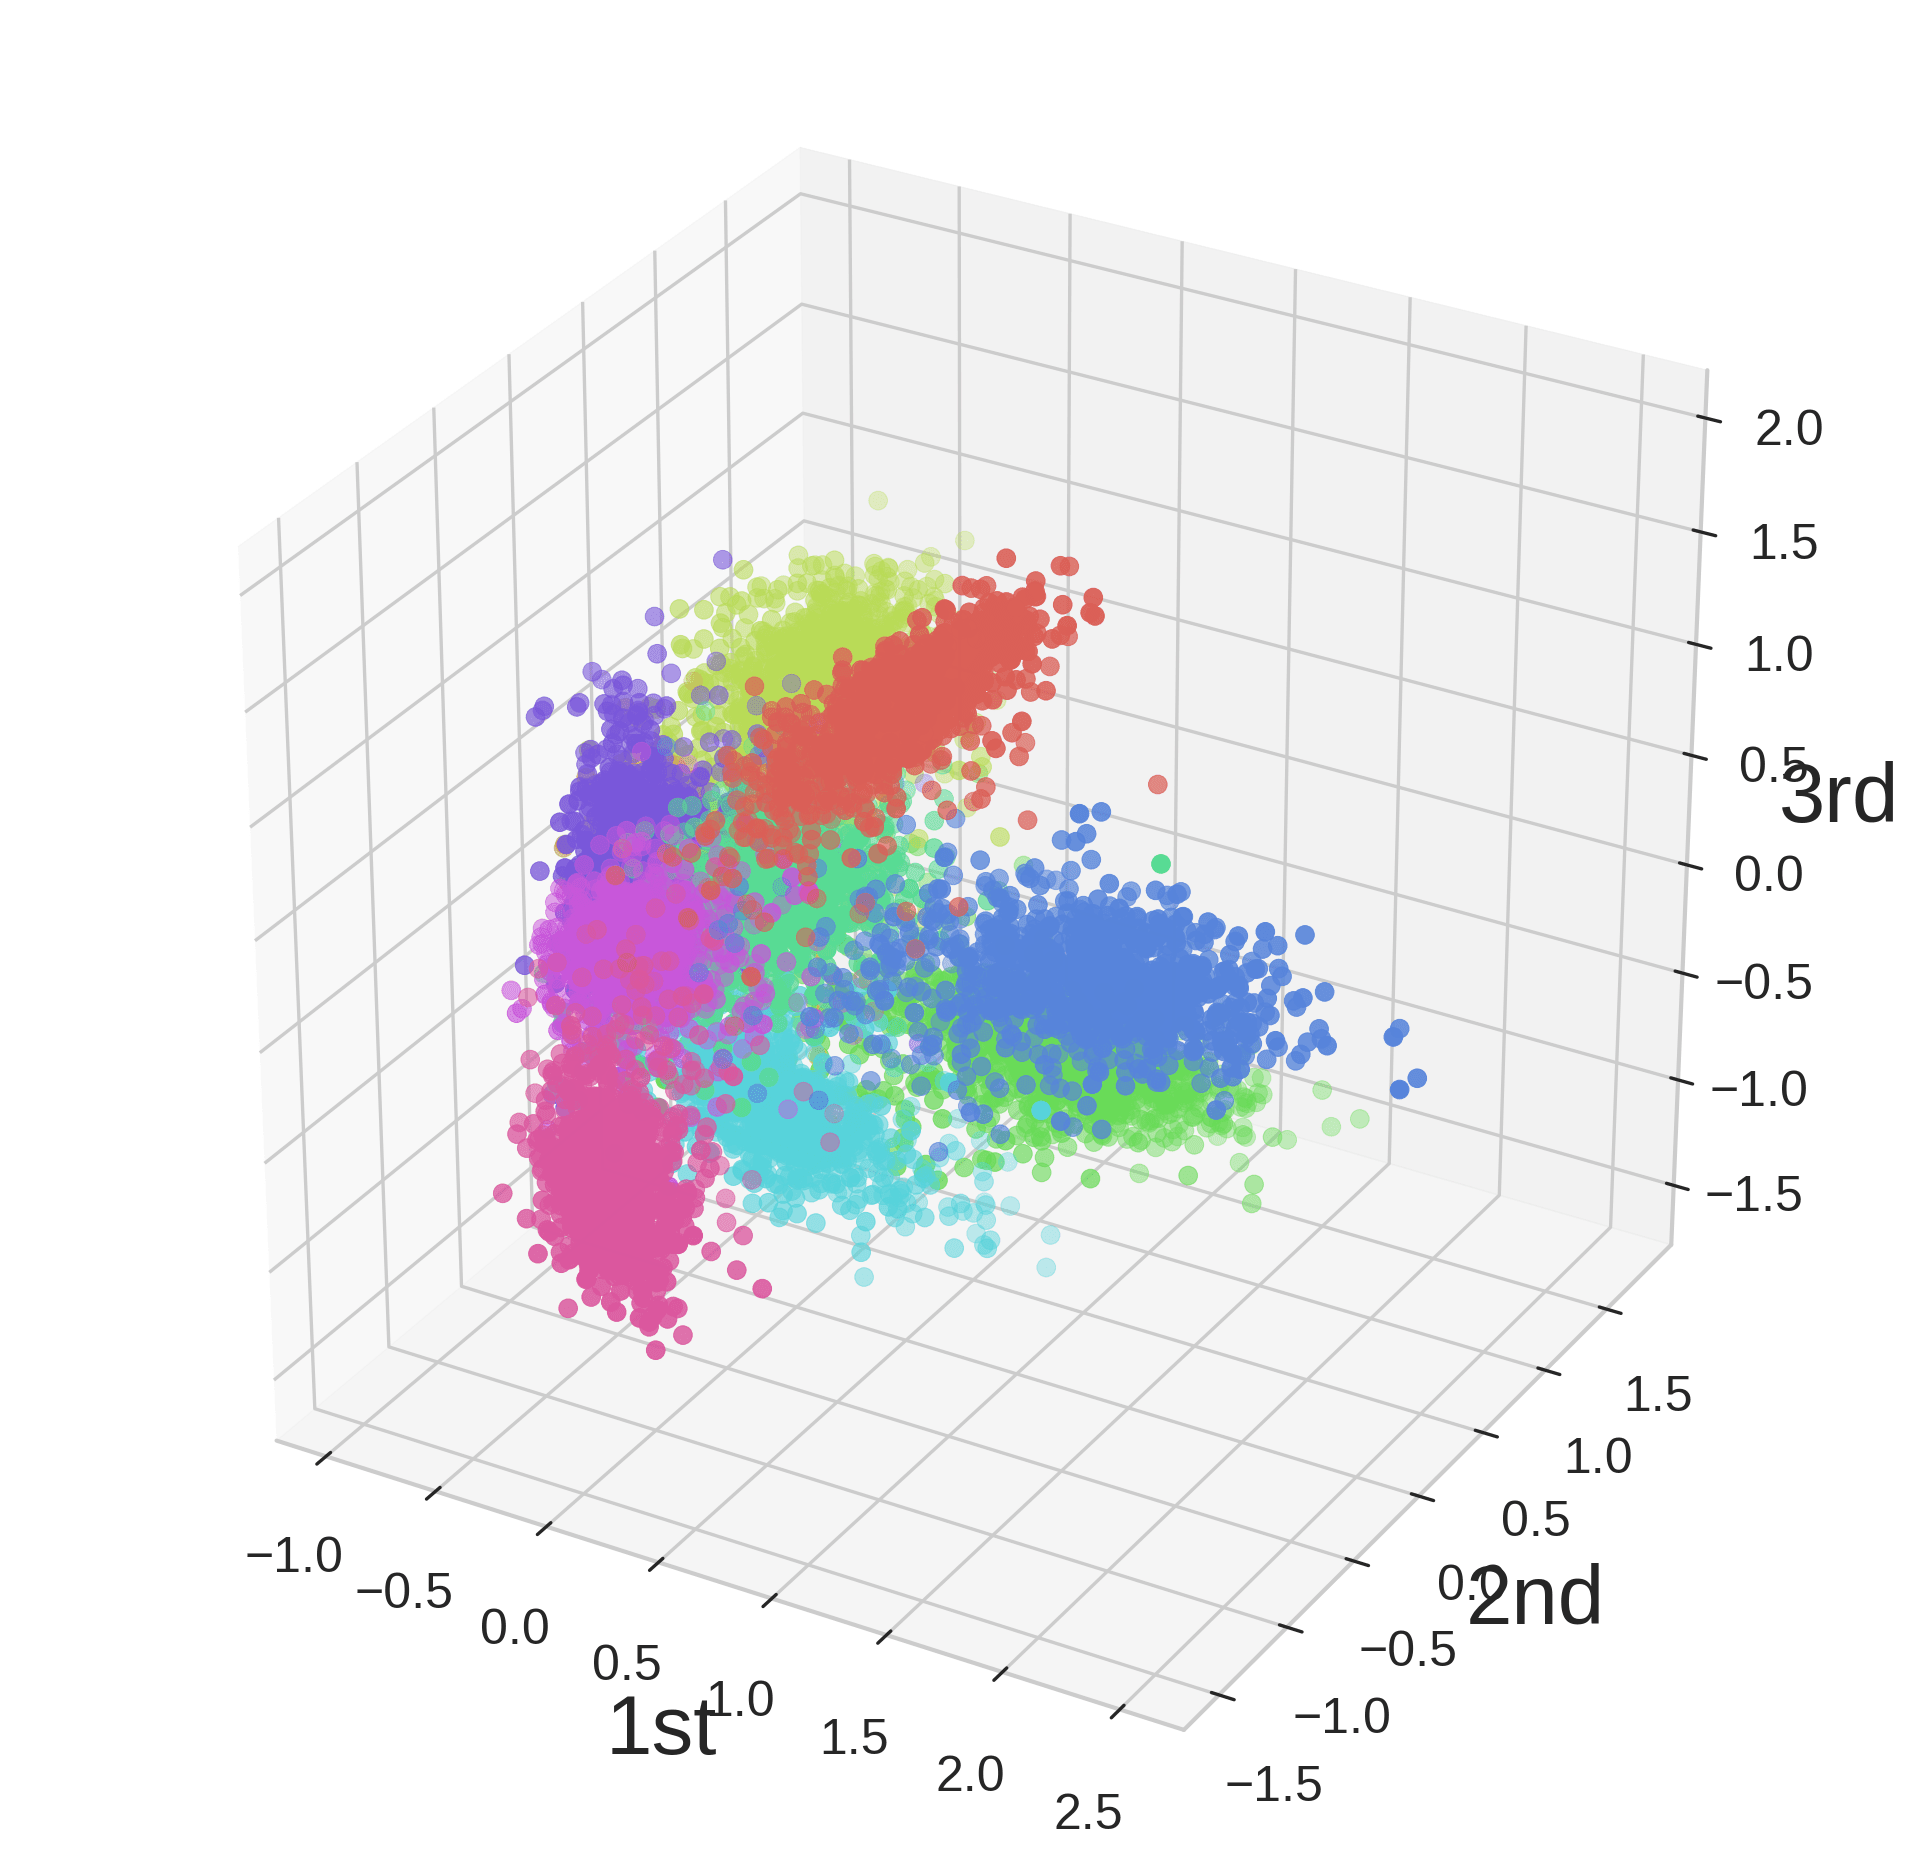
\includegraphics[width=4.5cm]{vr_fc5.png} }}%
    \qquad\qquad\qquad
    \subfloat[VR (After ReLU)]{{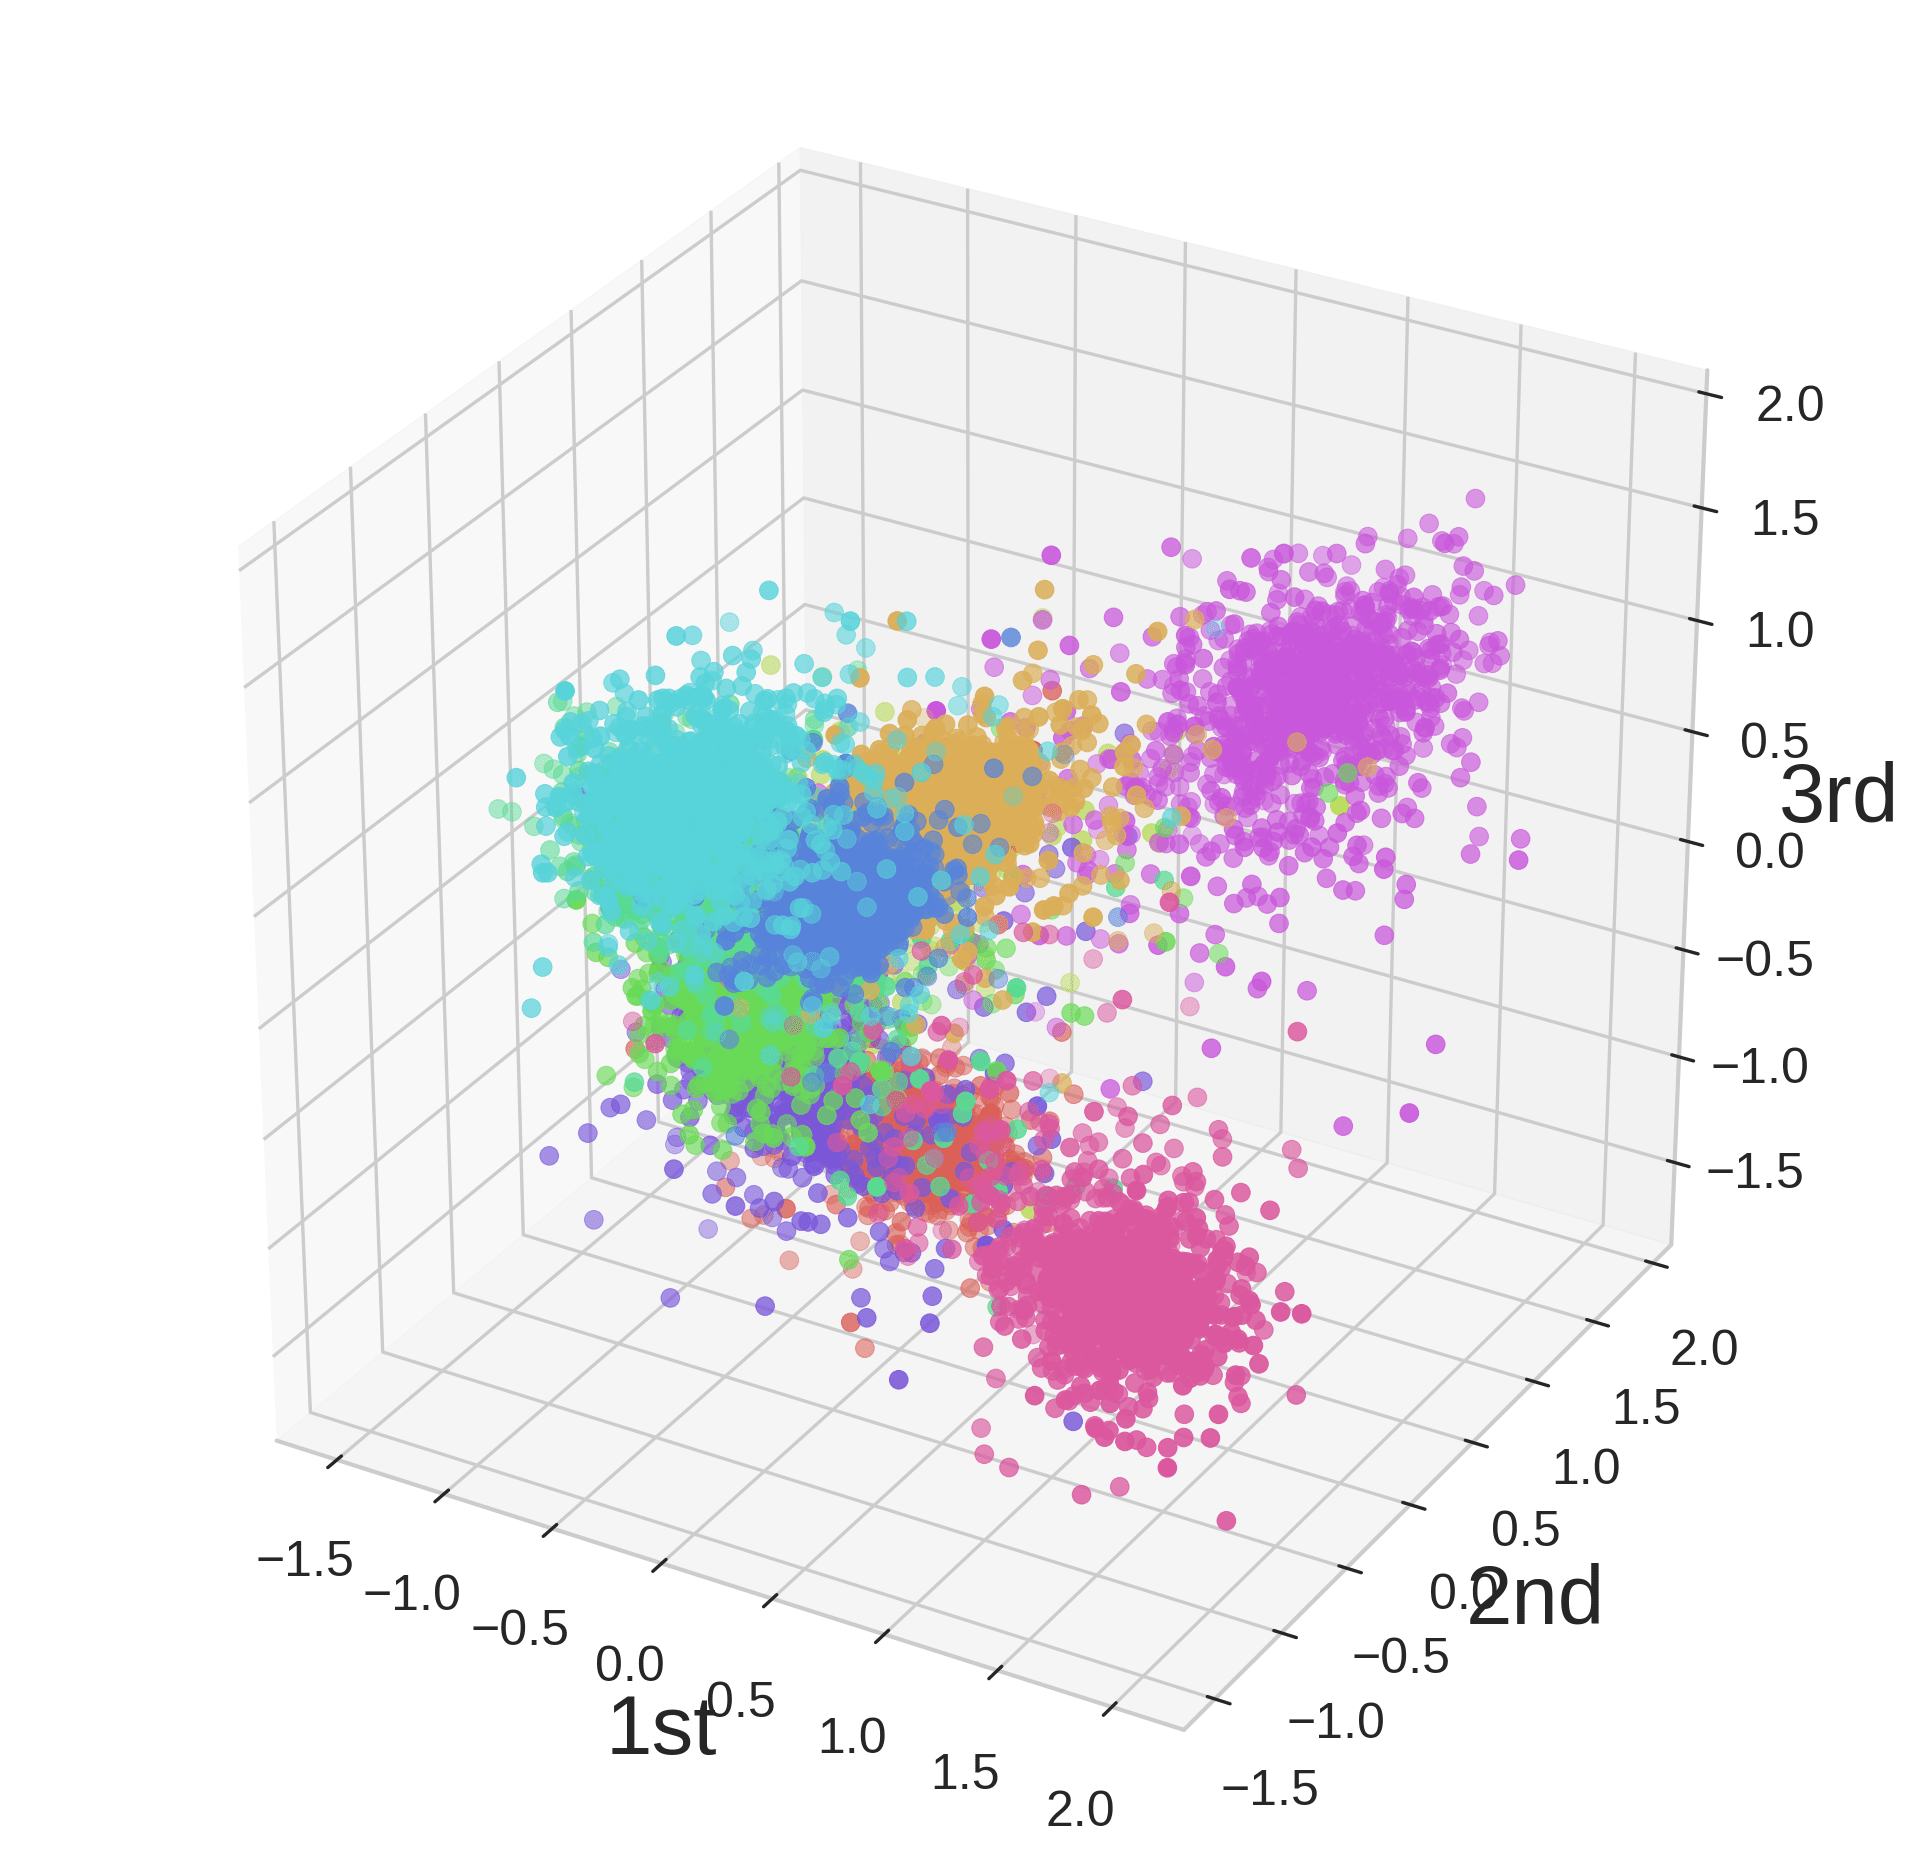
\includegraphics[width=4.5cm]{vr_fc5a.png} }}  
    
    \qquad\subfloat[cw-VR (Before ReLU)]{{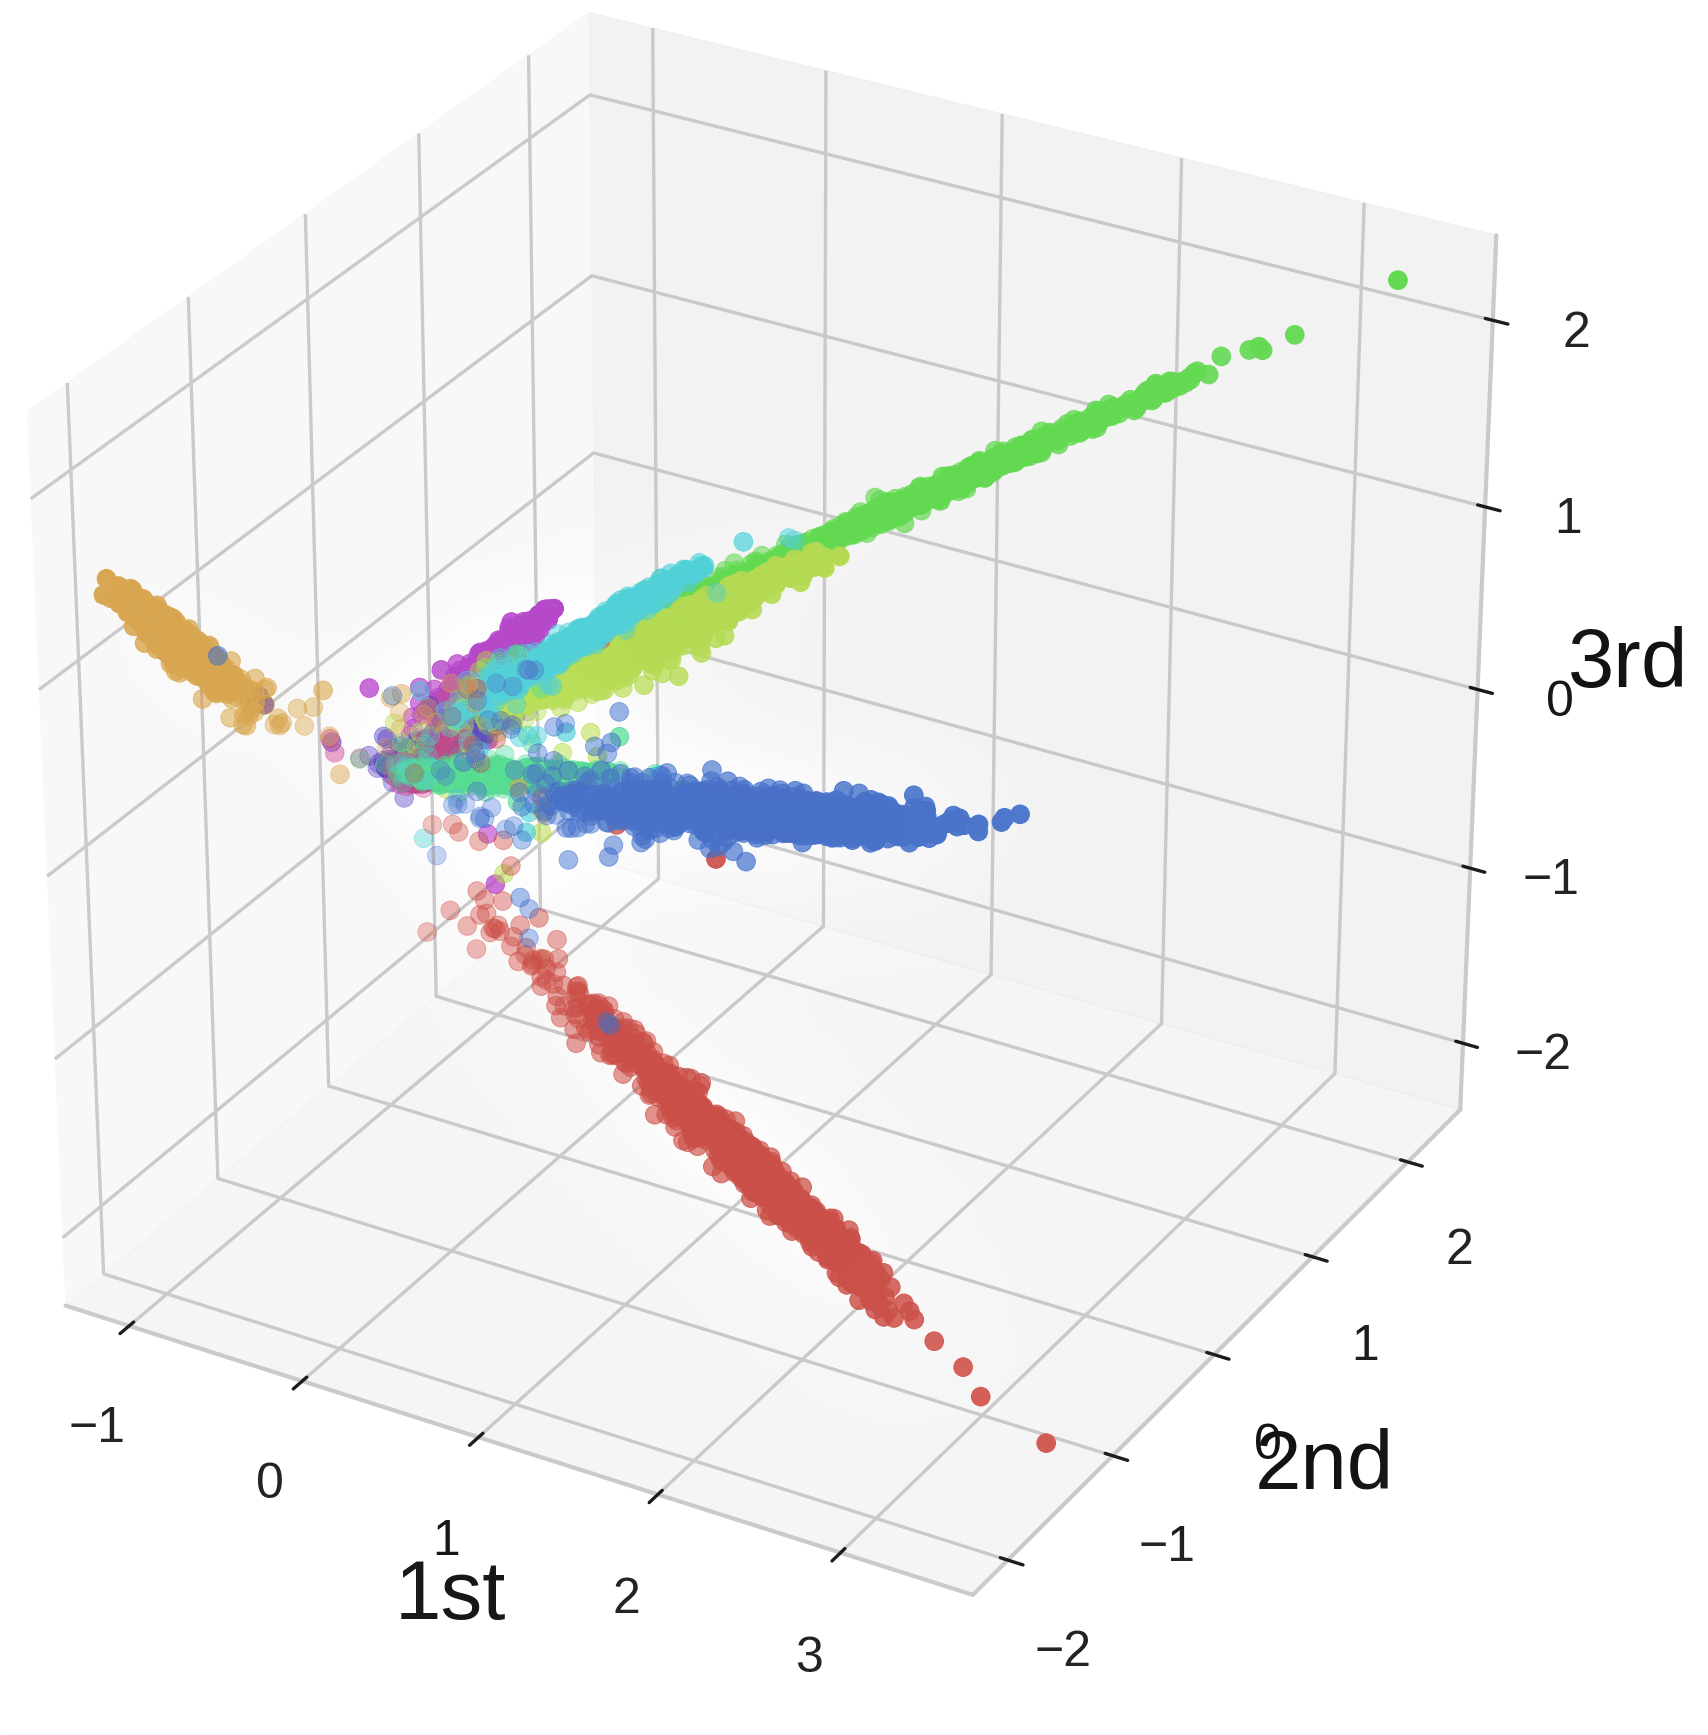
\includegraphics[width=4.cm]{cw_vr_fc5.png} }}%
    \qquad\qquad\qquad\qquad
    \subfloat[cw-VR (After ReLU)]{{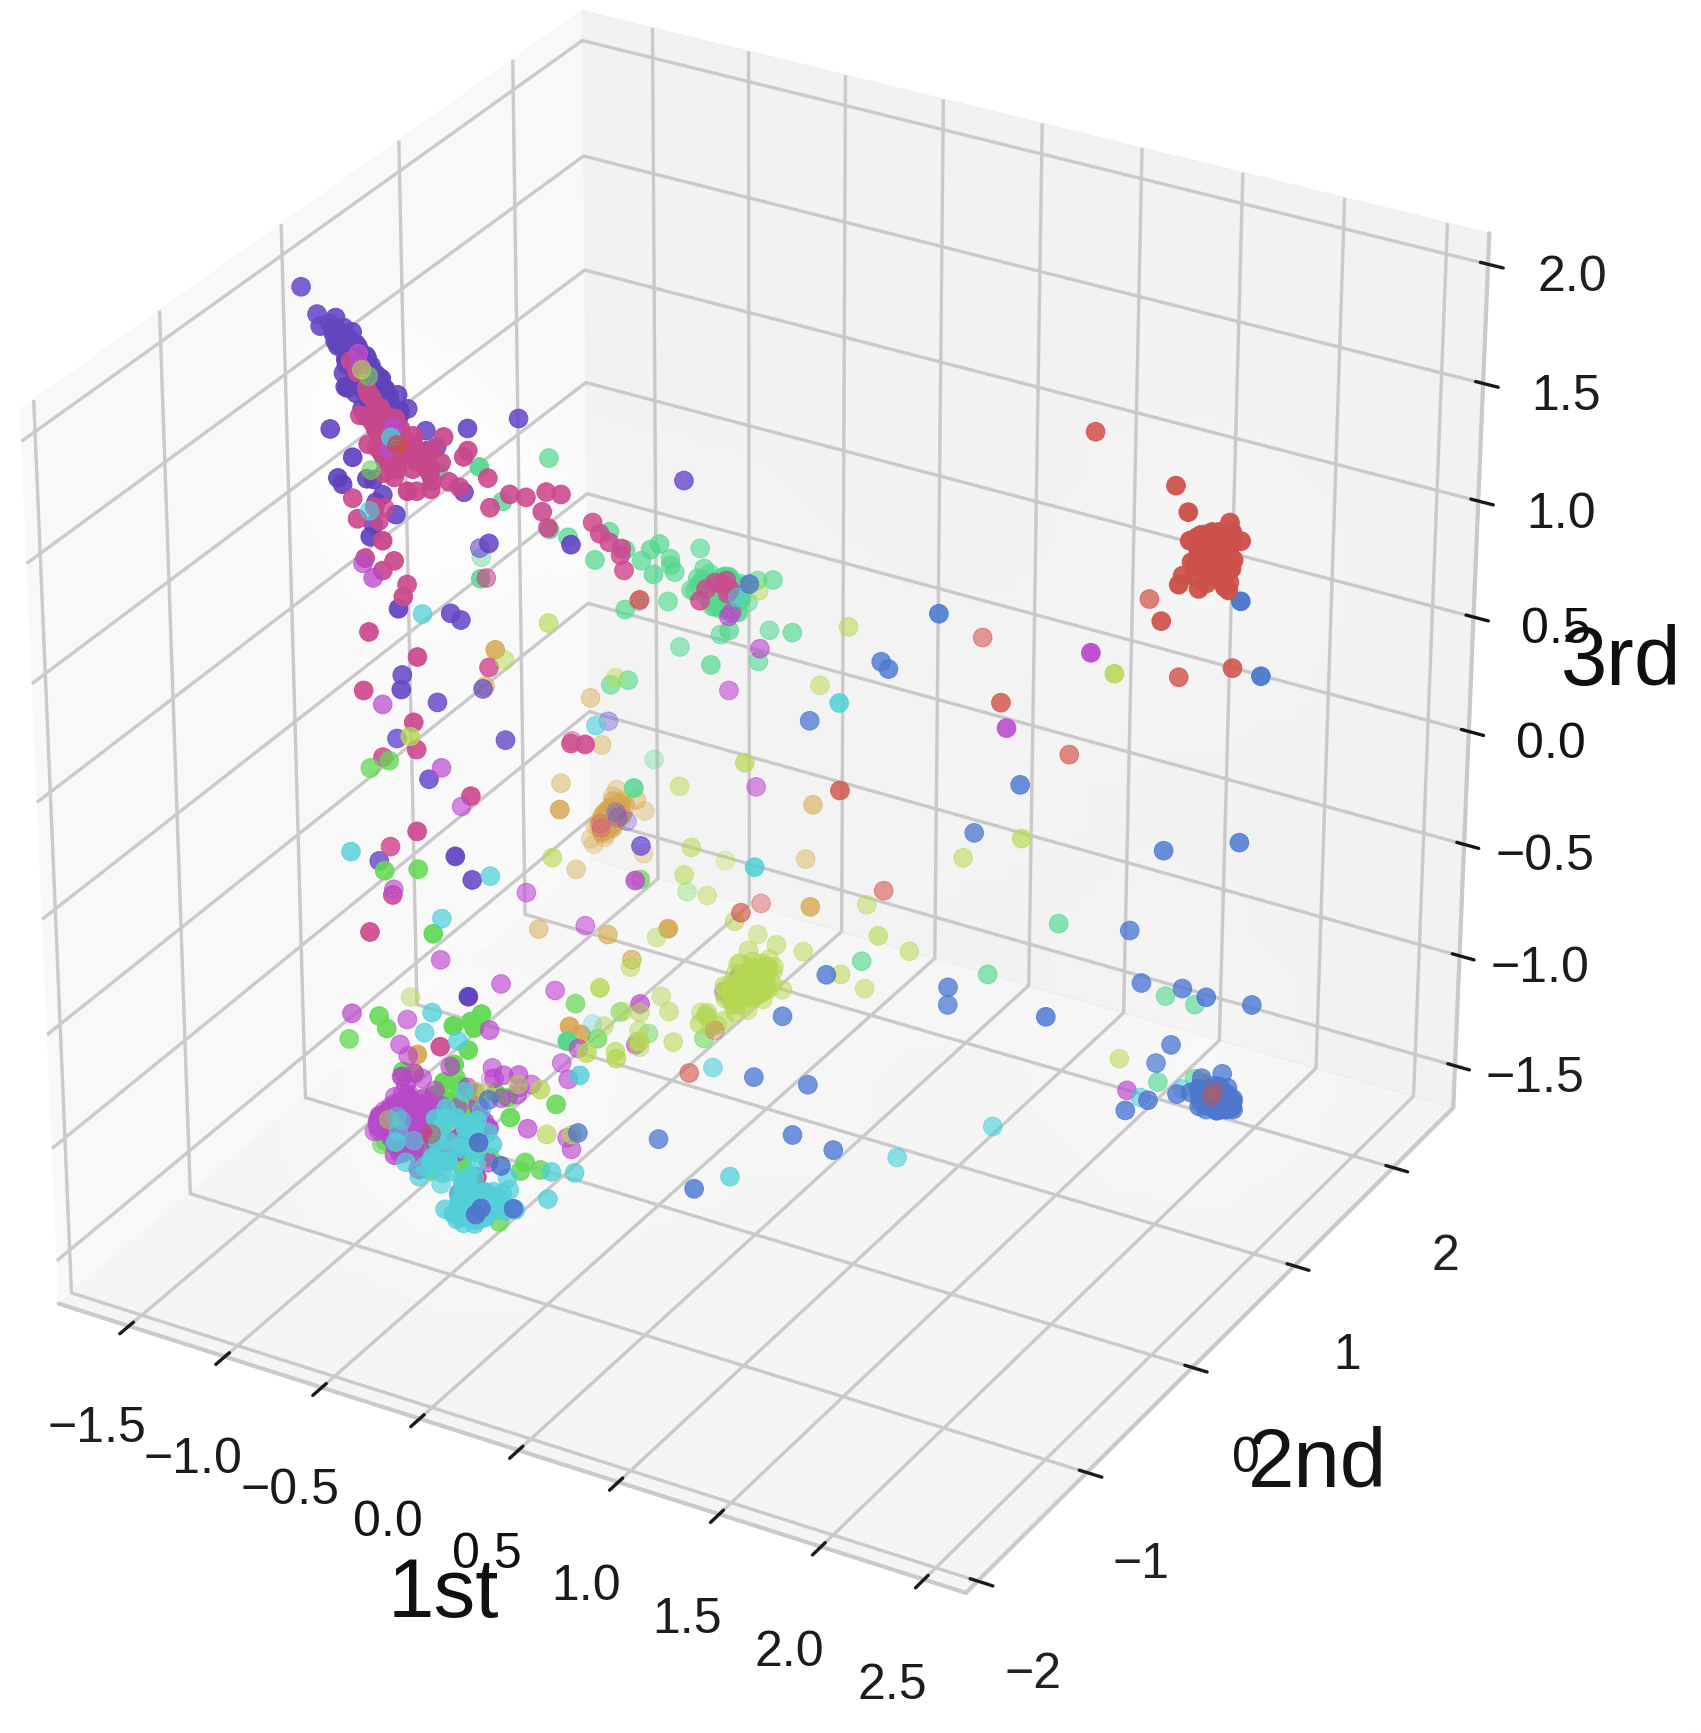
\includegraphics[width=4.cm]{cw_vr_fc5a.png} }}  
    \captionsetup{labelformat=empty}
\caption{Figure 5: The top three principal components of learned representations (representation regularizers).}%
    \label{fig:pca_2}%
\end{figure}


\clearpage

\section*{D\quad Layer Dependency}

\begin{figure}[htbp]
% \vskip 0.1in
\begin{center}
\centerline{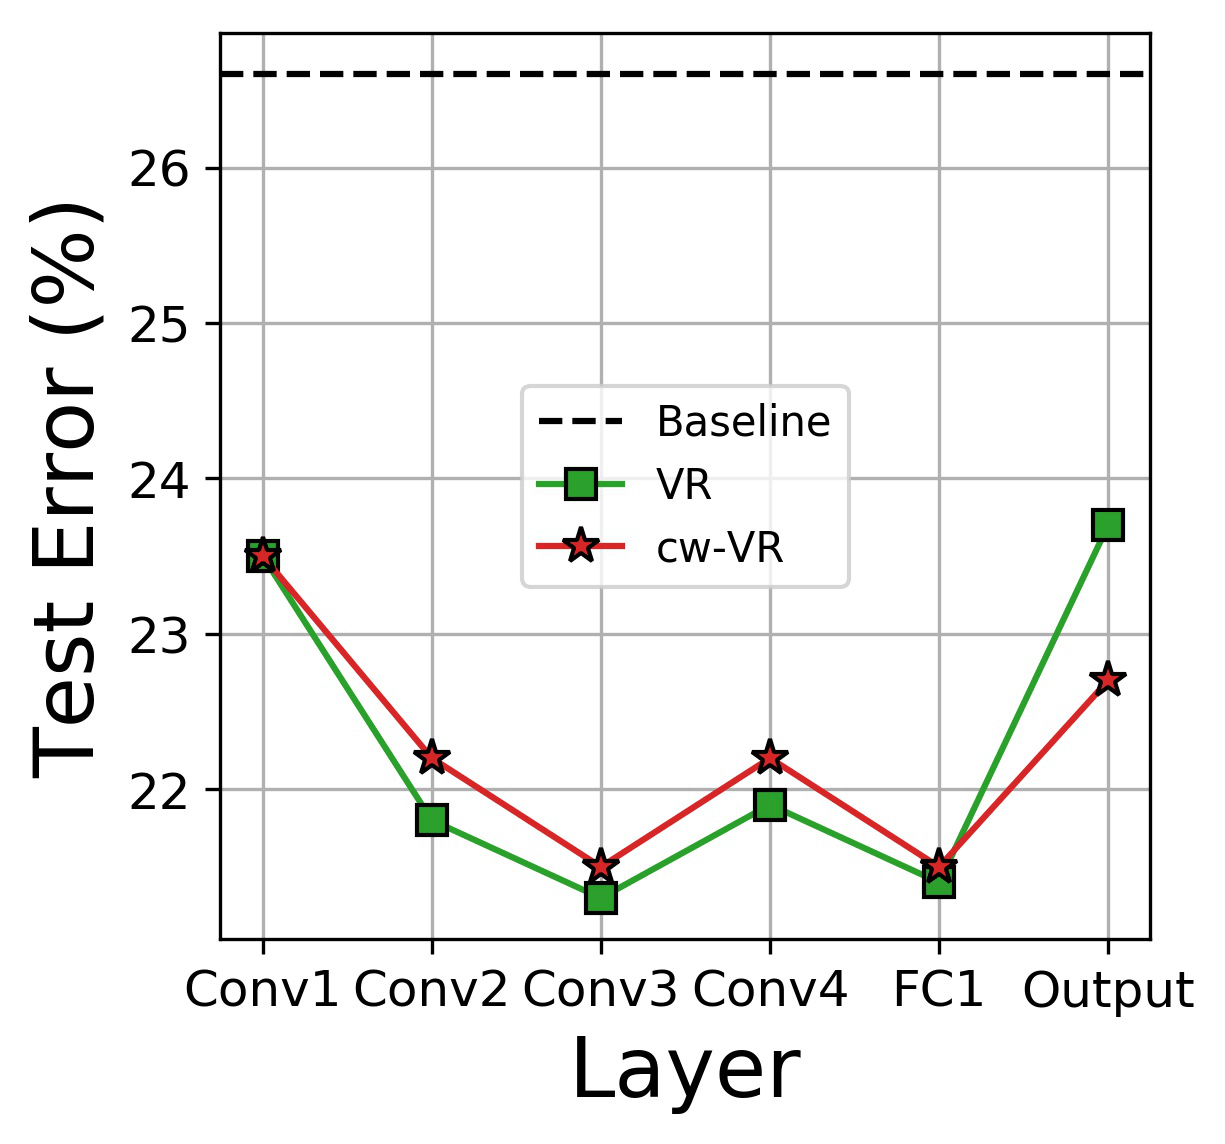
\includegraphics[width=4.1cm]{layer_cifar10.png}}
\captionsetup{labelformat=empty}
\caption{Figure 6:Layer dependency of representation regularizers on CIFAR-10 CNN model. The x-axis indicates layers where regularizers are applied. CR and cw-CR are excluded because of the high computational burden of applying them to the convolutional layers.}
\label{fig:layer_dependency_cifar10}
\end{center}
% \vskip -0.3in
\end{figure}

% \begin{table}[t]
% \caption{Mean Squared Error of Autoencoders. Standard deviation values are not included in the table because all of them are less than $10^{-4}$.} 
% \begin{center}
% \vskip -0.1in
% \begin{tabular}{cc}
% \hline
% Regularizer & Mean Squared Error                       \\ \hline
% Baseline    & $3.67 \times 10^{-3}  $                        \\
% L1W         & $3.64 \times 10^{-3}  $                        \\ 
% L2W         & $3.67 \times 10^{-3}  $                        \\ \hline
% cw-VR       & $2.50 \times 10^{-3}  $                        \\
% VR          & $2.39 \times 10^{-3}  $                        \\
% cw-CR       & $3.60 \times 10^{-3}  $                        \\
% CR          & $3.75 \times 10^{-3}  $                        \\ \hline
% \end{tabular}
% \label{table:autoencoder}
% \end{center}
% \vskip -0.15in
% \end{table}


% \section*{C. Feature Visualization}
% See page 3.

% \begin{figure}[t]
% \vskip -0.6in
%     \centering
%     \subfloat[Baseline (Autoencoder)]{{\includegraphics[width=4cm]{feature_none.png} }}%
%     \qquad\qquad\qquad
%     \subfloat[Baseline (MLP)]{{\includegraphics[width=4cm]{mlp_feature_none.png} }} \\
    
%     \subfloat[cw-VR (Autoencoder)]{{\includegraphics[width=4cm]{feature_cw_vr.png} }}%
%     \qquad\qquad\qquad
%     \subfloat[cw-VR (MLP)]{{\includegraphics[width=4cm]{mlp_feature_cw_vr.png} }} \\ 
    
%     \subfloat[VR (Autoencoder)]{{\includegraphics[width=4cm]{feature_vr.png} }}%
%     \qquad\qquad\qquad
%     \subfloat[VR (MLP)]{{\includegraphics[width=4cm]{mlp_feature_vr.png} }} \\ 
    
%     \subfloat[cw-CR (Autoencoder)]{{\includegraphics[width=4cm]{feature_cw_cr.png} }}%
%     \qquad\qquad\qquad
%     \subfloat[cw-CR (MLP)]{{\includegraphics[width=4cm]{mlp_feature_cw_cr.png} }} \\ 
    
%     \subfloat[CR (Autoencoder)]{{\includegraphics[width=4cm]{feature_cr.png} }}%
%     \qquad\qquad\qquad
%     \subfloat[CR (MLP)]{{\includegraphics[width=4cm]{mlp_feature_cr.png} }} 
%     \caption{Learned Features using Representation Regularizers.}%
%     \label{fig:feature_all}%
% \end{figure}



% \end{document}
